%% LyX 2.1.4 created this file.  For more info, see http://www.lyx.org/.
%% Do not edit unless you really know what you are doing.
\documentclass[12pt,english]{report}
\usepackage{charter}
\renewcommand{\familydefault}{\rmdefault}
\usepackage[T1]{fontenc}
\usepackage[a4paper]{geometry}
\geometry{verbose,tmargin=2.5cm,bmargin=2.5cm,rmargin=2.5cm}
\setcounter{secnumdepth}{3}
\setcounter{tocdepth}{3}
\setlength{\parskip}{\medskipamount}
\setlength{\parindent}{0pt}
\usepackage{color}
\usepackage{babel}
\makeatletter

\makeatother
\usepackage{float}
\usepackage{graphicx}
\usepackage{setspace}
\usepackage{nomencl}
% the following is useful when we have the old nomencl.sty package
\providecommand{\printnomenclature}{\printglossary}
\providecommand{\makenomenclature}{\makeglossary}
\makenomenclature
\onehalfspacing
\usepackage[unicode=true,
 bookmarks=true,bookmarksnumbered=true,bookmarksopen=true,bookmarksopenlevel=1,
 breaklinks=true,pdfborder={0 0 1},backref=false,colorlinks=true]
 {hyperref}
\hypersetup{
 linkcolor=black, citecolor=red, urlcolor=blue, filecolor=blue, pdfstartview=XYZ}

\makeatletter

%%%%%%%%%%%%%%%%%%%%%%%%%%%%%% LyX specific LaTeX commands.
%% Because html converters don't know tabularnewline
\providecommand{\tabularnewline}{\\}

%%%%%%%%%%%%%%%%%%%%%%%%%%%%%% User specified LaTeX commands.
% the pages of the TOC is numbered roman
% and a pdf-bookmark for the TOC is added
\pagenumbering{roman}

%\let\myTOC\tableofcontents
%\renewcommand\tableofcontents{%
 % \pdfbookmark[1]{\contentsname}{}
 % \myTOC
 % \cleardoublepage  }

%*****Chapter style******
\usepackage[Glenn]{fncychap}
\ChNameVar{\large}
\ChTitleAsIs
\ChTitleVar{\bfseries\Huge}

%*****Header style*******
\usepackage{fancyhdr}
 
\pagestyle{fancy}

\fancyhf{}
\fancyhead[LE,RO]{\thepage}
\fancyhead[RE,LO]{\footnotesize\nouppercase{\leftmark}}

%\renewcommand{\chaptermark}[1]{\markboth{#1}{}}

\renewcommand{\headrulewidth}{0,5pt}

%****Glossaire Title*****
\renewcommand{\nomname}{Glossaire}

\makeatother

\begin{document}
\noindent \begin{titlepage}
\begin{center}
% Upper part of the page
\begin{minipage}{0.4\textwidth}   Réf : xx/xx  \end{minipage}
\begin{minipage}{0.4\textwidth} \begin{flushright} A.U. : 2014-2015 \end{flushright}\end{minipage}
\rule[0.5ex]{1\columnwidth}{1pt}\\[0.5cm]
\textsc{\large{Université de Sousse}}\\
\textsc{\large{Ecole Nationale d'Ingénieurs de Sousse}}\\
%\includegraphics[width=0.3\textwidth]{logo.png}\\[-0.5cm]
\Large{Rapport de Projet de Fin d'Etudes}\\[0.5cm]
\normalsize{Présenté en vue de l'obtention du diplôme d'}\\
\Large{ \bfseries{Ingénieur en Génie .....}}\\
\normalsize{Option ...}\\[0.6cm]
\rule[0.5ex]{1\columnwidth}{1pt}\\[0.5cm]
{ \huge \bfseries Conception et développement d'une application }\\[0.5cm]
\rule[0.5ex]{1\columnwidth}{1pt}\\[2cm]
% Author and supervisor
\begin{minipage}{0.4\textwidth} \begin{flushleft} \large \emph{Réalisé par:}\\ Prénom~\textsc{Nom} \end{flushleft} \end{minipage} \begin{minipage}{0.5\textwidth} \begin{flushright} \large \emph{Encadré par:} \\  Mr.~Prénom~\textsc{Nom} \end{flushright} \end{minipage}
\vfill
% Bottom of the page 
\end{center}
\end{titlepage}


\newpage
~\\
~\\
~\\
~\\
\begin{center}
To my family and all my beloved.
\end{center}



\chapter*{Acknowledgements}

I would like to express my gratitude towards my university's supervisor, Mr. Taha Ben Salah, and my company's supervisor Mr. Richard Lindberg for supporting me during my internship and for all the knowledge and experience they shared with me.
I would also like to thank all my professors for teaching me and helping me achieve my goals.


\tableofcontents{}

\listoffigures


\listoftables



\chapter*{Abstract}
My graduation project consists in creating a web application that contains listings of hotels, restaurants and any place available in the Google places API and allows registered users to create reviews about these places as well as rate these places following some specific criteria like the use of renewable energy and the use of recyclable materials..
The web app also provides a REST API that is being used by a mobile app developed separately. Part of the project also consists of deploying the app to the cloud.

\section*{Keywords}
Python - Django - Sustainable Tourism - REST API - Amazon Web Services - Ratings



\pagenumbering{arabic} 



\chapter*{Introduction}

The internet is full of tourism platforms that list hotels, restaurants and similar tourism related services. To name a few of them we can cite as notable examples: Tripadvisor, Trivago and Kayak. There is literally tens of these platforms, from different countries and in different shapes and colours. However all of the existing platforms only let users write "general" reviews about the listed places, and the visitors can only distinguish between those places based on either the prices or the "general" reviews.
It turns out that there’s also a market for people who are interested in "sustainable tourism" and don’t mind paying more for an eco-friendly vacation. Sustainable tourism is defined as "tourism that respects local people, the traveller, cultural heritage and the environment" by UNESCO, you think of it as "fairtrade" and "organic" but for the travel sector.

One Planet Rating (OPR) was created to fill this void and serve this portion of tourists by listing the same places while focusing on sustainability instead of price.
One Planet Rating is a newly founded social startup based in Stockholm, with a portion of its team members working remotely (partially including myself). The startup is in it’s very early stages, it’s main product/service is the web application described in this report.The company’s service isn’t released to the public yet.
The company thrives to have an impact and aims, with its services, to help achieve some of the United Nations’ Sustainable Development Goals (UN SDGs) like:
\begin{itemize}

\item UN SDG 8: "Promote sustained, inclusive and sustainable economic growth, full and productive employment and decent work for all".
\item UN SDG 15: Protect, restore and promote sustainable use of terrestrial ecosystems, sustainably manage forests, combat desertification, and halt and reverse land degradation and halt biodiversity loss"
\item UN SDG 13: "Take urgent action to combat climate change and its impacts by regulating emissions and promoting developments in renewable energy.
\end{itemize}
OPR is a tourism platform that is sustainability focused, it allows people from around the world to rate and review touristic services based on how much they respect the earth.
The long term goal of OPR is to promote the movement of sustainable tourism and incite people to be more responsible during their trips, and eventually help protect the environment and the community.
OPR also emphasizes on transparency as it doesn’t participate in writing the reviews and ratings, it only provides a playground for all people to express themselves freely.


In this report we’ll briefly cover the state of the art and market analysis of the project.
In the first chapter we’ll go through the requirements and specifications.
The second chapter covers the design aspect of the project.
The third chapter covers the development and deployment aspects of the project.


\chapter{State of the art}


Many online tourism platforms exist today, we can consider these platforms as “indirect competitors” because they offer an alternative functionality to OPR, but what makes the most difference is the target market.
Some of these major platforms are Tripadvisor(Fig.1), Trivago(Fig.2) and Momondo(Fig.3).
As shown in the following screenshots, all of those platforms focus on the general ratings and the price.
They offer very similar functionalities but in different layouts.

\begin{figure}[H]
\centering
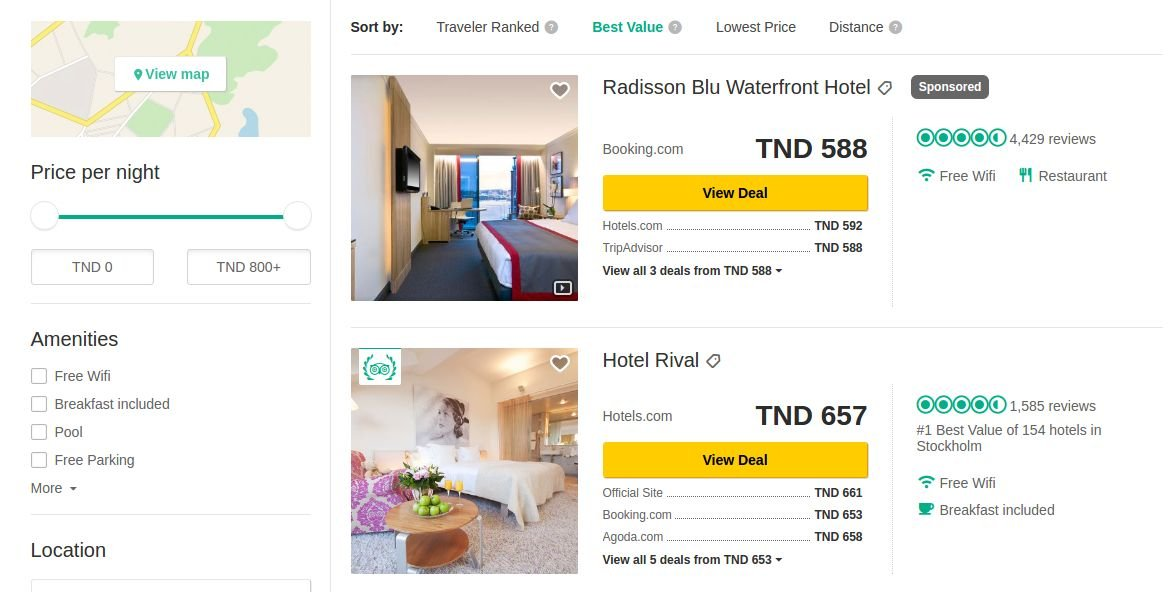
\includegraphics[width=15cm]{tripadvisor.jpg}
\caption{screenshot of Tripadvisor}
\end{figure}


Trip advisor, which is the world leader in the tourism sector provides hotel booking and listing of tourism establishments. The company is based in the United States, and it also offers other related services like tourism focused forums. The platform also allows users to search for and book flight tickets.

\begin{figure}[H]
\centering
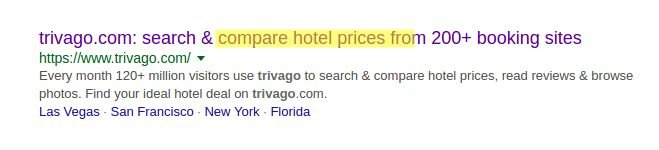
\includegraphics[width=15cm]{trivago.jpg}
\caption{screenshot of search results for Trivago}
\end{figure}

In contrast, the Germany based company, Trivago, only focuses on hotels. Trivago is the leader hotel search engine in Germany. Though trivago only lists hotels, it is owned by Expedia, which owns and operates more than 200 websites that offer diverse services in the tourism and travel sectors.


\begin{figure}[H]
\centering
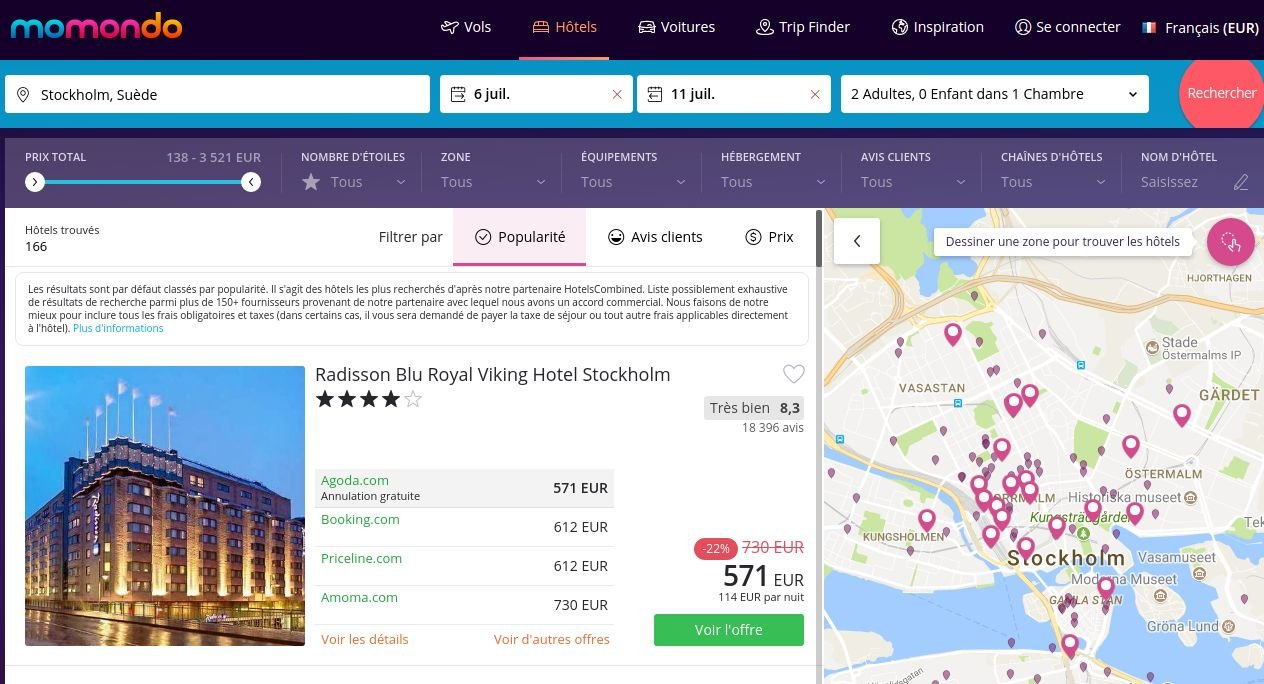
\includegraphics[width=15cm]{momondo.jpg}
\caption{screenshot of Momondo}
\end{figure}

Momondo is also a similar service which, in addition to listing hotels, also provides flight booking and car rental services. Another interesting thing about Momondo is that it’s based in Scandinavia, and this makes of it a local competitor.

Another thing to note is that most of these “indirect competitors” are booking websites while OPR is not. OPR’s goal is to promote the sustainable places and punish the unsustainable ones.





The following table shows more in detail the difference between OPR and the above-mentioned competitors:
\begin{table}[H]
\centering
\begin{tabular}{|l|l|l|l|l|}
\hline
Funtionality                       & Tripadvisor & Trivago & Momondo & OPR \\ \hline
Search hotels                      & YES         & YES     & YES     & YES \\ \hline
Search restaurants                 & YES         & NO      & NO      & YES \\ \hline
Search activities and other places & YES         & NO      & NO      & YES \\ \hline
Search for flights                 & YES         & NO      & YES     & NO  \\ \hline
Search for flights                 & NO          & NO      & YES     & NO  \\ \hline
Booking service                    & YES         & YES     & YES     & NO  \\ \hline
General ratings                    & YES         & YES     & YES     & YES \\ \hline
Sustainabilityratings              & NO          & NO      & NO      & YES \\ \hline
\end{tabular}
\caption{comparison of tourism platforms}
\label{my-label}
\end{table}




Another category of competitors includes magazines, blogs and expert websites ( like shown in Fig.4) that promote some specific sustainable places. Those are also indirect competitors because they rely on experts’ advice on their reviews which tend to be not very trustworthy. OPR’s content will be completely user generated, because most people believe more in reviews created by peers and want to be part of the content creation. OPR will only be the intermediary between content creators and content consumers, and will not participate in content creation.

\begin{figure}[H]
\centering
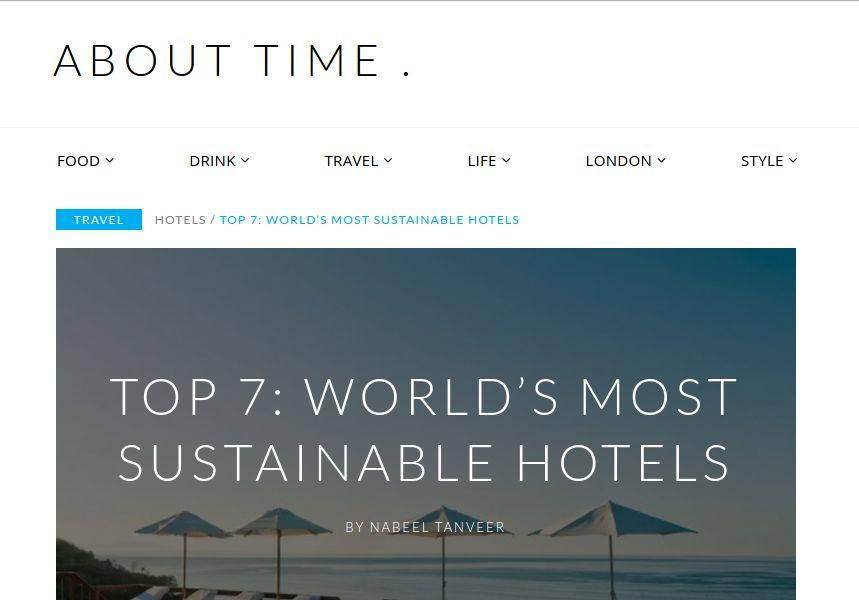
\includegraphics[width=15cm]{blog.jpg}
\caption{example of an expert blog}
\end{figure}


\section{Formalism}
During the work on this project we used the following formal methods:
\subsection*{UML}
We used UML (Unified Modeling Language)for describing and modeling the specifications of the project. UML is very flexible and versatile. UML is also one of the best choices for modeling because it is very popular and widely used across the globe, which makes of it easier to grasp by other people. Most software engineers are probably familiar with it.
\subsection*{Agile scrum}
We used the agile scrum methodology because it is the most convenient method to the project. Every week we have a sprint where we define the goals of that week from the backlog. This methodology turned to be very efficient, especially that the project consists in developing a prototype, which requires continuous thinking and customization. Agile scrum allowed us to customize the project while working on it.


\chapter{Specifications}
\section{Actors}
\subsection{Internal actors}
\paragraph{User}
~\\
Anybody who accesses OPR Ratings via App or Web is a User. As opposed to “Member” (see
below) this does not require any log-on, or creation of a OPR Profile.
A User can search for specific places and read reviews of those places.


\paragraph{Member}
~\\
OPR Members are Users who sign up to use OPR’s services with a Profile. A User needs to be
logged in, to be acting as a Member.
A member can do everything a User can do, in addition to the ability of posting their own
reviews and ratings.

\paragraph{Manager}
~\\
In addition to the permissions that a Member has, an Admin has the permission to Create,
Read, Update and Delete (CRUD) Ads, reviews and rating categories.

\paragraph{Admin}
~\\
The admin is responsible of managing the users, he has the permission to CRUD users.


\subsection{External actors}


\paragraph{Google places service}
~\\
Google places API is called for every search to look for relevant places based on provided location.\\
The API provides us with :\\
Basic information (Name, address..), Photo, Google’s place\_id (unique identifier)

\paragraph{Google maps service}
~\\
Google Maps API provides us with a map pointing at the specific location based on the location’s place\_id we retrieve from Google Places API


\paragraph{Gmail service}
~\\
Google’s Gmail is used to send the emails to users.


\section{Functionalities' overview}

The main functionality of the platform is to allow members to read and post reviews and ratings
about some specific places. Obviously this implies that they need to be able to register and login
to the platform. Users should also be able to search for a specific place by a keyword. And since
OPR is all about sustainability-related reviews, the platform offers the possibility to rate
establishments based on multiple criteria.
The platform also has a mobile app, and this implies that the web based app should provide an
API to supply the mobile app with the data.

\begin{figure}[H]
\centering
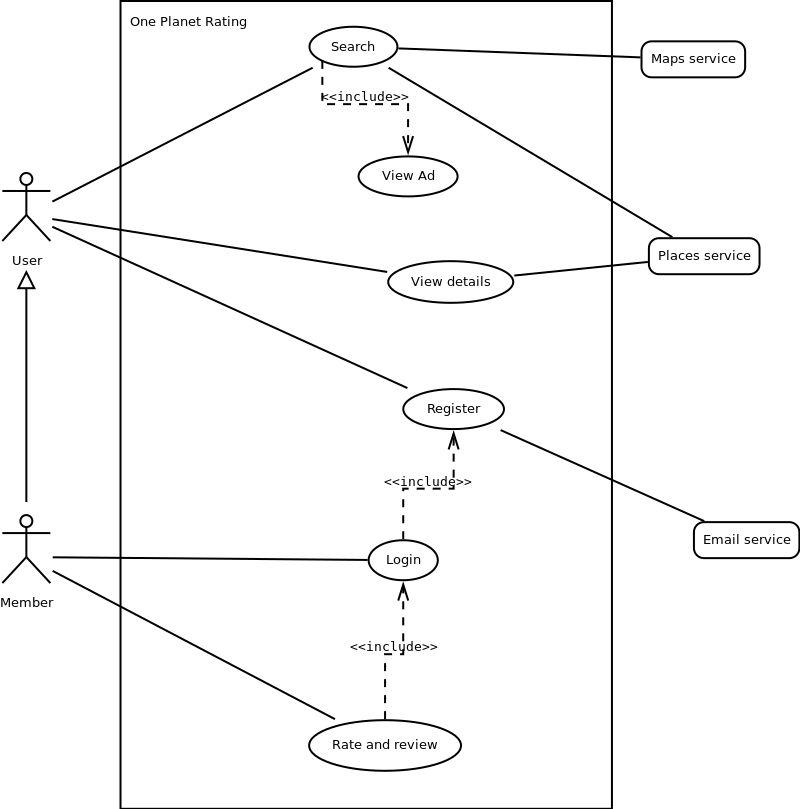
\includegraphics[width=15cm]{generalUseCase.jpg}
\caption{general usecase diagram}
\end{figure}

As shown in the use case diagram, any user can use the app to search and view the details of a
place. The search functionality pulls data from Google places service, and shows a map using
Google maps service.
When a user registers, he becomes a member. During the registration process Gmail service is
used to send a confirmation email.
The member can then login to his profile and becomes able to rate and review places.

\subsection{Register}

\begin{figure}[H]
\centering
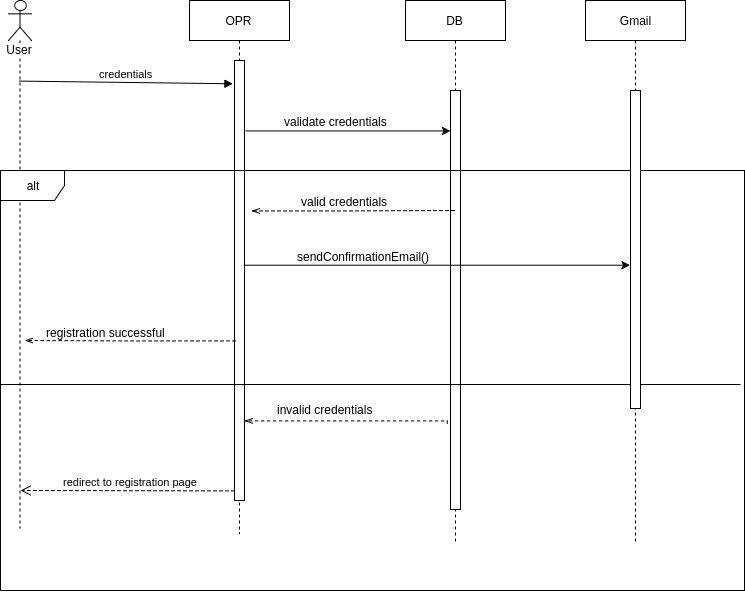
\includegraphics[width=15cm]{registerSequence.jpg}
\caption{registration sequence diagram}
\end{figure}

\begin{table}[H]
\centering
\begin{tabular}{|l|l|}
\hline
Title             & Registration                                                                                                                                                                                                                                                                                    \\ \hline
Author            & Moetaz Ben Charrada                                                                                                                                                                                                                                                                             \\ \hline
Version           & 1.0                                                                                                                                                                                                                                                                                             \\ \hline
Objectives        & Allows users to register and create an account                                                                                                                                                                                                                                                  \\ \hline
Actors            & User - OPR - Gmail                                                                                                                                                                                                                                                                              \\ \hline
Pre-conditions    & \begin{tabular}[c]{@{}l@{}}The user should be on the registration page\\ The user must not be already registered.\end{tabular}                                                                                                                                                                  \\ \hline
Post-conditions   & The user becomes registered (member)                                                                                                                                                                                                                                                            \\ \hline
Story             & \begin{tabular}[c]{@{}l@{}}1. The user enters his username\\ 2. The user enters his email\\ 3. The user enters his password\\ 4. The user re-enters his password\\ 5. The user submits the form\end{tabular}                                                                                    \\ \hline
Alternative story & \begin{tabular}[c]{@{}l@{}}The functionality is accessed through the\\ mobile app instead of a browser.\end{tabular}                                                                                                                                                                            \\ \hline
Exceptional story & \begin{tabular}[c]{@{}l@{}}If the user enters an email that’s already in the DB,\\  the user will be prompted to enter a different email.\\ If the user enters a password that’s not \\ compliant to the security constraints, he will\\ be prompted to enter a different password\end{tabular} \\ \hline
\end{tabular}
\caption{Registration description}
\label{my-label}
\end{table}


\subsection{Login}

\begin{figure}[H]
\centering
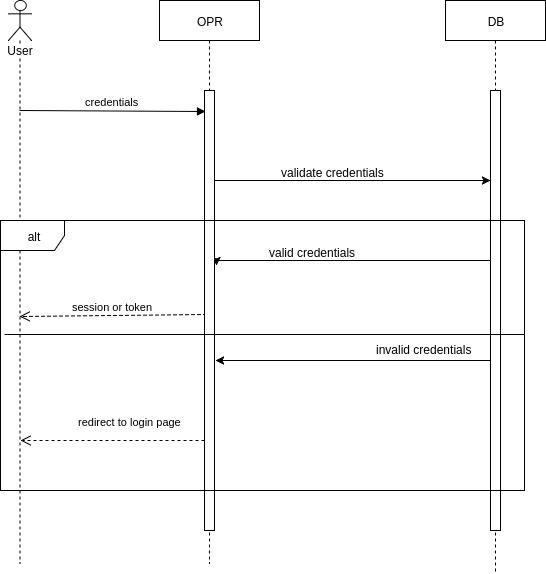
\includegraphics[width=15cm]{loginSequence.jpg}
\caption{login sequence diagram}
\end{figure}

\begin{table}[H]
\centering
\begin{tabular}{|l|l|}
\hline
Title             & Login                                                                                                                                      \\ \hline
Author            & Moetaz Ben Charrada                                                                                                                        \\ \hline
Version           & 1.0                                                                                                                                        \\ \hline
Objectives        & Allows users to login and access his account                                                                                               \\ \hline
Actors            & User - OPR                                                                                                                                 \\ \hline
Pre-conditions    & \begin{tabular}[c]{@{}l@{}}The user should be a registered member.\\ The user must not be already logged in.\end{tabular}                  \\ \hline
Post-conditions   & \begin{tabular}[c]{@{}l@{}}The user becomes authenticated.\\ The user can then post reviews.\end{tabular}                                  \\ \hline
Story             & \begin{tabular}[c]{@{}l@{}}1. The user enters his username\\ 2. The user enters his password\\ 3. The user submits the form\end{tabular}   \\ \hline
Alternative story & \begin{tabular}[c]{@{}l@{}}The functionality is accessed through the\\ mobile app instead of a browser.\\ (Through the REST API)\end{tabular} \\ \hline
Exceptional story & \begin{tabular}[c]{@{}l@{}}If the user enters incorrect credentials, he will\\ be prompted to try to login again.\end{tabular}             \\ \hline
\end{tabular}
\caption{login description}
\label{my-label}
\end{table}

\newpage~

\begin{figure}[H]
\centering
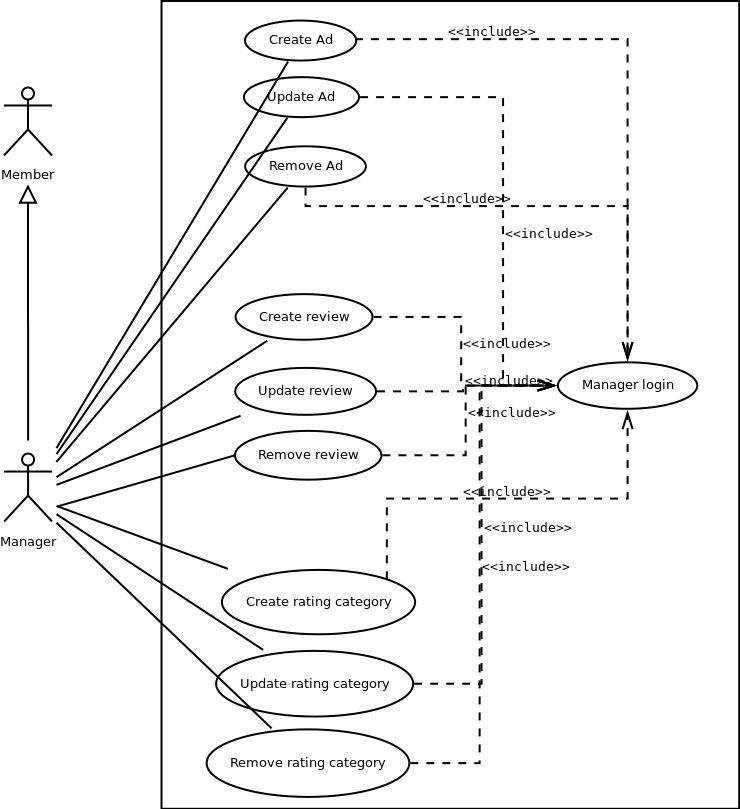
\includegraphics[width=15cm]{managerUseCase.jpg}
\caption{manager usecase diagram}
\end{figure}

A manager, is a member with additional privileges. An admin can create, update and delete:
ads, reviews and rating-categories.


\begin{figure}[H]
\centering
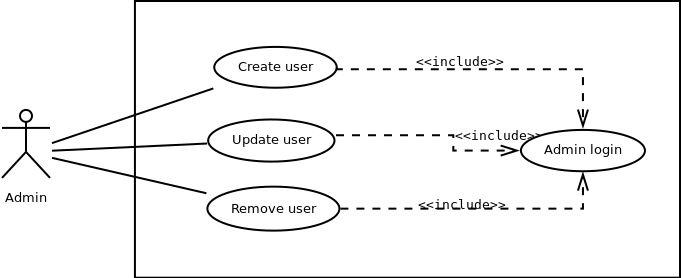
\includegraphics[width=15cm]{adminUseCase.jpg}
\caption{admin usecase diagram}
\end{figure}


\chapter{Design \& architecture}
\section{Physical architecture}

\begin{figure}[H]
\centering
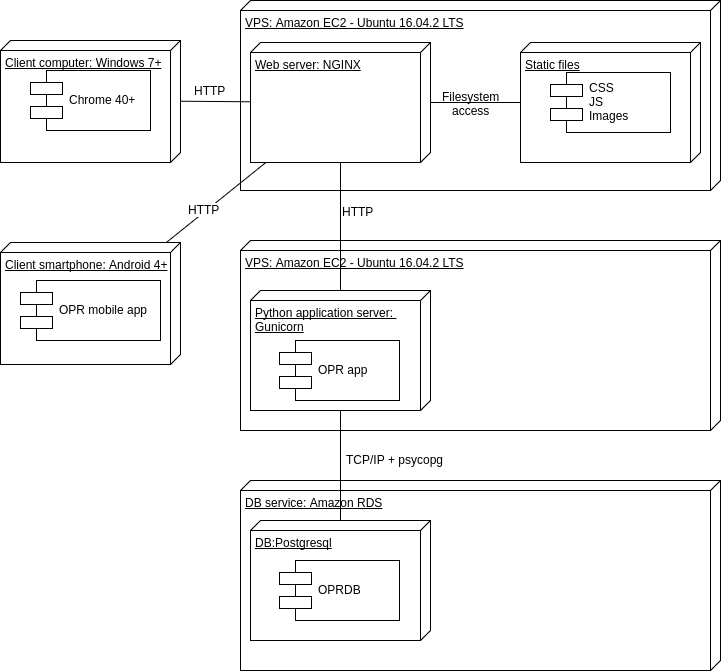
\includegraphics[width=15cm]{physicalArchitecture.png}
\caption{The app's physical architecture}
\end{figure}

\section{Logical architecture}

The architecture used is a mix of MVC + 3 Tiers.

\paragraph{3 Tiers}
~\\
3 Tiers was used to separate the data, logic and the client from each other. Each of those three
tiers is a separate, standalone entity. This provides more security, because if one of the tiers
gets attacked the other tiers remain intact. This also provides some sort of interoperability
because we can change one of the tiers without touching the other ones.

\paragraph{MVC}
~\\
MVC architecture was used in the server level. MVC architecture facilitates code visibility and
maintainability because the architecture is well known and one can easily predict and
understand the functionality of each of its components. MVC also has the advantage of loose
coupling, which also offers interoperability as explained in the example of 3 Tiers above.


\begin{figure}[H]
\centering
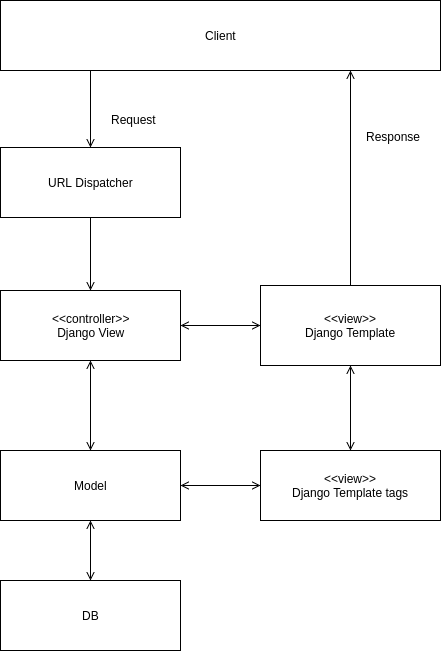
\includegraphics[width=12cm]{logicalArchitecture.png}
\caption{The app's logical architecture}
\end{figure}


\section{Modular architecture}

\begin{figure}[H]
\centering
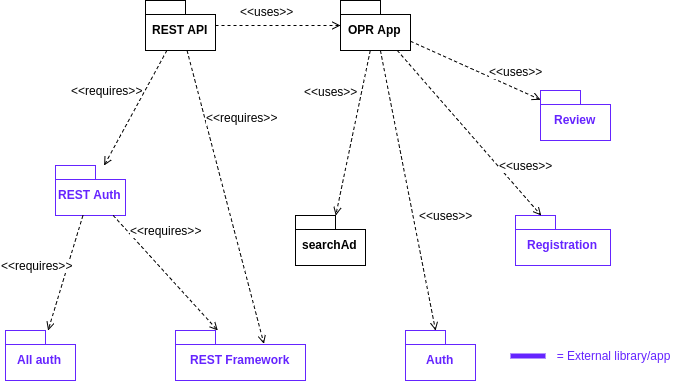
\includegraphics[width=15cm]{modularArchitecture.png}
\caption{The app's modular architecture}
\end{figure}

During my work on the project I tried my best to reuse existing code instead of re-writing what
already exists and is ready to use. Thus Most of the modules shown in the diagram are external
libraries.
My work consists of creating the following modules:
OPR App, REST API and searchAd.

\section{Modules}

\subsection{searchAdModule}
This is a standalone library that offers the possibility to create and show ads either from a local
source (the user’s DB) or from an external source (like Google Adsense).



\begin{figure}[H]
\centering
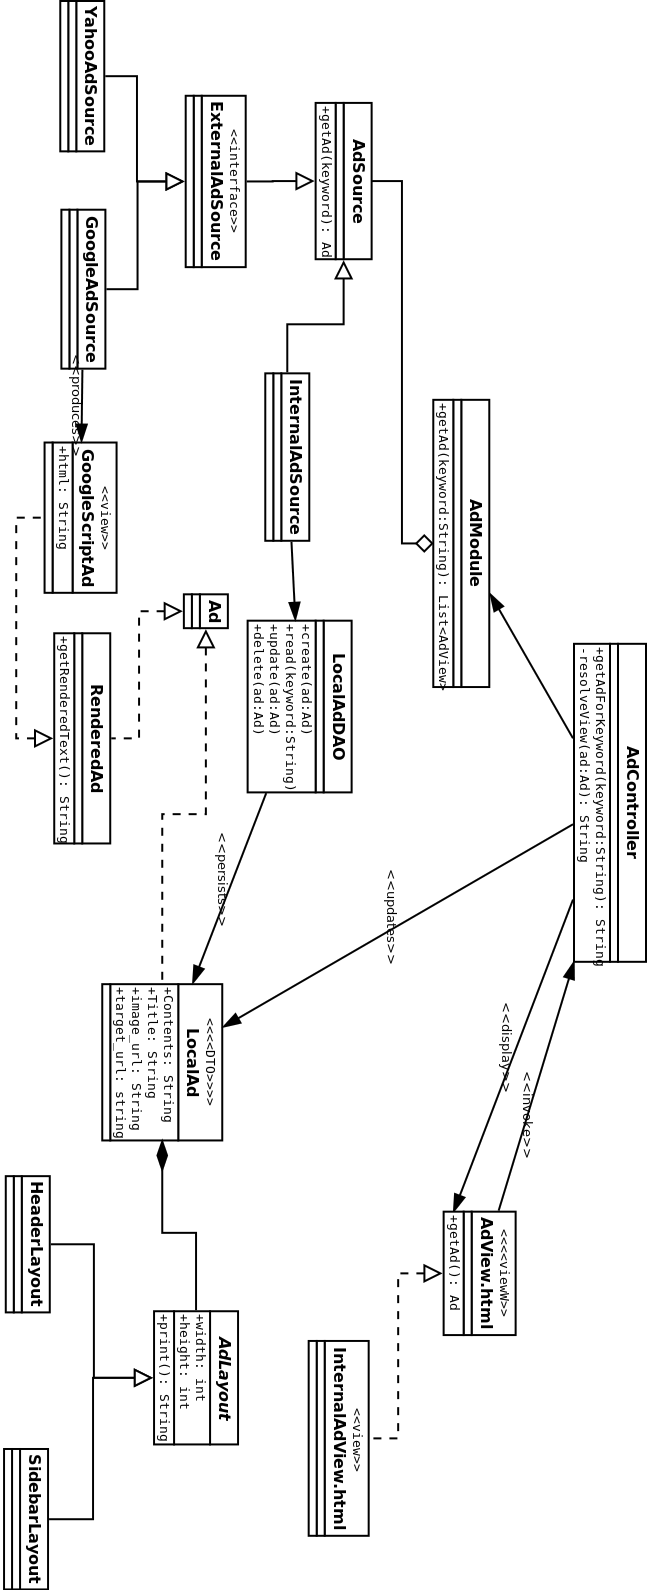
\includegraphics[width=10cm]{searchAdClass.png}
\caption{searchAd class diagram}
\end{figure}

The searchAd module is designed following the MVC architecture.
The AdController is the entrypoint for the module, it allows the user to get an ad based on a
keyword. It also contains a private method resolveView() that shows the ad in html format to be
directly injected in the view.\\
The ExternalAdSource allows to get ads from external sources like Google AdWords. It’s made
in a way to make it easily extensible with other external sources. In fact all we have to do is
create a new class inheriting the ExternalAdSource class and containing the url to the ads
service.\\
In case the ads are not pulled from an external source, they’re stored in the local database as
LocalAd. The LocalAd model contains a title, content, target\_url and image\_url.


\subsection{OPR app module}
this is the main app, it contains the business logic for searching and rating places. It’s also
where most of the other libraries are integrated and linked together.

\paragraph{Search}~\\

\begin{figure}[H]
\centering
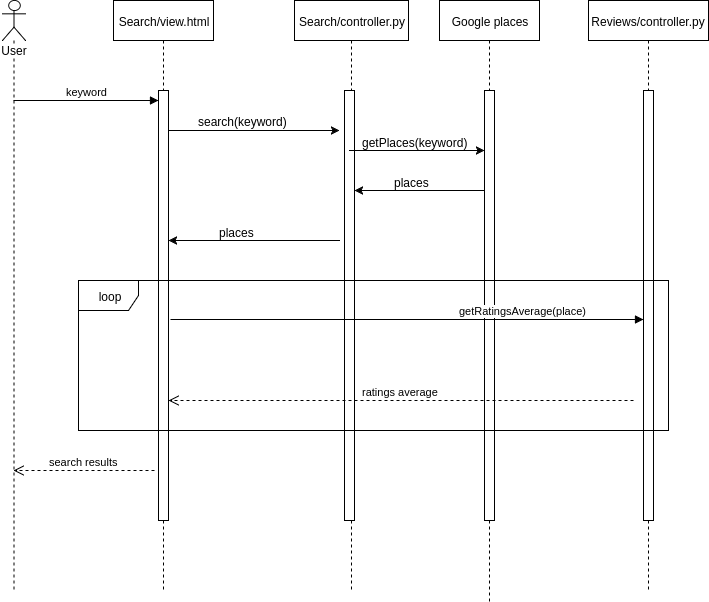
\includegraphics[width=15cm]{searchSequence.png}
\caption{search sequence diagram}
\end{figure}


\begin{table}[H]
\centering
\begin{tabular}{|l|l|}
\hline
Title             & Search                                                                                                                                                                              \\ \hline
Author            & Moetaz Ben Charrada                                                                                                                                                                 \\ \hline
Version           & 1.0                                                                                                                                                                                 \\ \hline
Objectives        & Allows users to search for a specific place.                                                                                                                                        \\ \hline
Actors            & User - OPR - Places service                                                                                                                                                         \\ \hline
Pre-conditions    & \begin{tabular}[c]{@{}l@{}}The user should be on a page where there's\\ a search bar.\end{tabular}                                                                                  \\ \hline
Post-conditions   & \begin{tabular}[c]{@{}l@{}}The user finds places related to his keywords,\\ and may click to check the details of that\\ place.\end{tabular}                                        \\ \hline
Story             & \begin{tabular}[c]{@{}l@{}}1. The user enters keywords related \\ to the place he's looking for\\ 2. The user selects the type of place\\ 3. The user submits the form\end{tabular} \\ \hline
Alternative story & \begin{tabular}[c]{@{}l@{}}The functionality is accessed through the\\mobile app instead of a browser.\\ (Through the REST API)\end{tabular}                                          \\ \hline
\end{tabular}
\caption{search description}
\label{my-label}
\end{table}



\paragraph{View details}~\\

\begin{figure}[H]
\centering
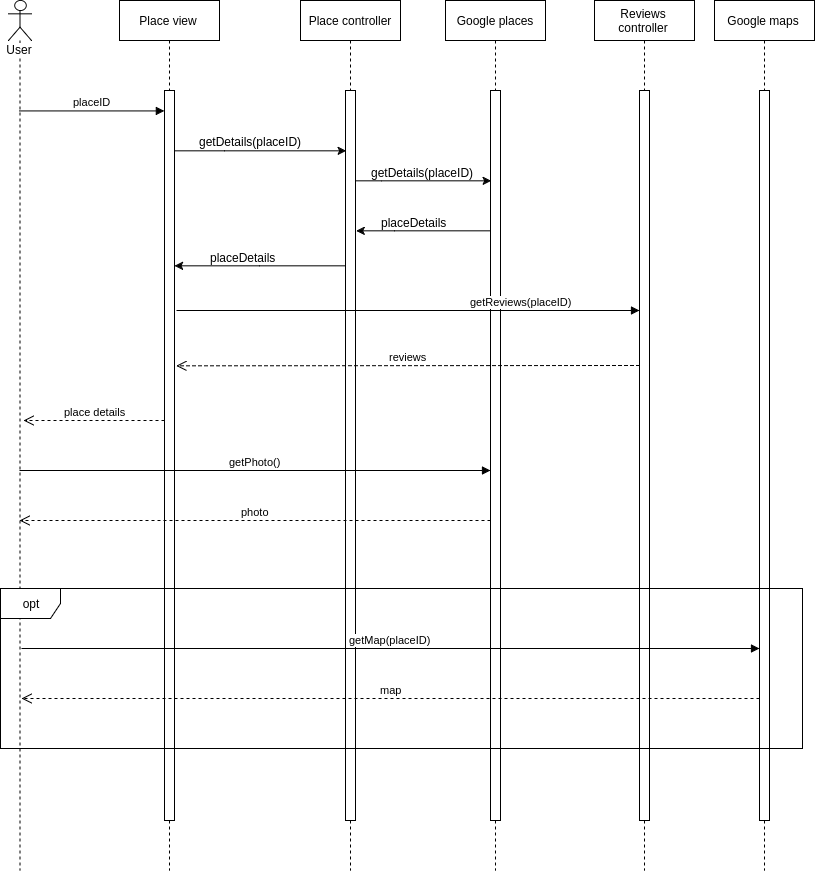
\includegraphics[width=15cm]{viewSequence.png}
\caption{view-details sequence diagram}
\end{figure}

\begin{table}[H]
\centering
\begin{tabular}{|l|l|}
\hline
Title             & View details                                                                                                                                                                                                                                                                                                                       \\ \hline
Author            & Moetaz Ben Charrada                                                                                                                                                                                                                                                                                                                \\ \hline
Version           & 1.0                                                                                                                                                                                                                                                                                                                                \\ \hline
Objectives        & \begin{tabular}[c]{@{}l@{}}Allows users to view the details and reviews\\ of a specific place\end{tabular}                                                                                                                                                                                                                         \\ \hline
Actors            & User - OPR - Places service - Maps service                                                                                                                                                                                                                                                                                         \\ \hline
Pre-conditions    & \begin{tabular}[c]{@{}l@{}}The user should have searched for the\\ place before.\end{tabular}                                                                                                                                                                                                                                      \\ \hline
Post-conditions   & \begin{tabular}[c]{@{}l@{}}The user sees the details and reviews of \\ the place and can possibly post a review about it.\end{tabular}                                                                                                                                                                                             \\ \hline
Story             & \begin{tabular}[c]{@{}l@{}}1. The user clicks on one of the places he found\\ in the search view.\\ 2. OPR app will then get the details of that\\  place from Google places service, get\\  the map from Google maps service.\\ 3. The data is combined with the local\\ reviews’ data and is sent back to the user.\end{tabular} \\ \hline
Alternative story & \begin{tabular}[c]{@{}l@{}}The functionality is accessed through the\\ mobile app instead of a browser.\\ (Through the REST API)\end{tabular}                                                                                                                                                                                      \\ \hline
\end{tabular}
\caption{view-details description}
\label{my-label}
\end{table}




\paragraph{Review a place}~\\

\begin{figure}[H]
\centering
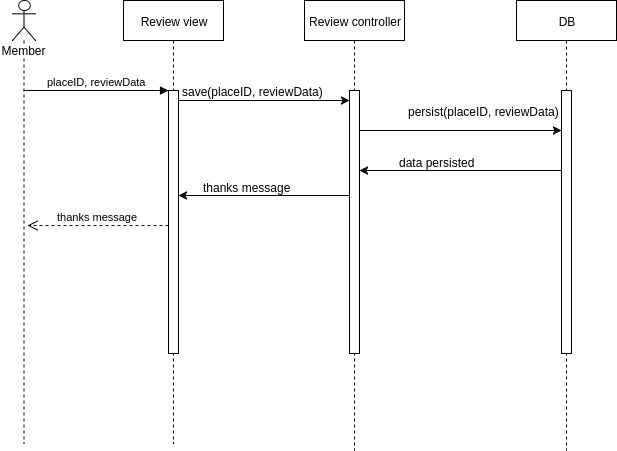
\includegraphics[width=15cm]{reviewSequence.png}
\caption{review a place sequence diagram}
\end{figure}


\begin{table}[H]
\centering
\begin{tabular}{|l|l|}
\hline
Title             & Review a place                                                                                                                                                                                           \\ \hline
Author            & Moetaz Ben Charrada                                                                                                                                                                                      \\ \hline
Version           & 1.0                                                                                                                                                                                                      \\ \hline
Objectives        & \begin{tabular}[c]{@{}l@{}}Allows users to post a review about a specific\\ place\end{tabular}                                                                                                           \\ \hline
Actors            & User - OPR                                                                                                                                                                                               \\ \hline
Pre-conditions    & \begin{tabular}[c]{@{}l@{}}The user should be authenticated to be able\\ to post a review.\end{tabular}                                                                                                  \\ \hline
Post-conditions   & \begin{tabular}[c]{@{}l@{}}The user creates a review.\\ The review becomes visible to the public.\end{tabular}                                                                                           \\ \hline
Story             & \begin{tabular}[c]{@{}l@{}}1.The user enters his review data \\ 2.The user submits the form. \\ 3.The review data is saved to the \\ database.\\ 4.A thanks message is shown to\\ the user.\end{tabular} \\ \hline
Alternative story & \begin{tabular}[c]{@{}l@{}}The functionality is accessed through the\\ mobile app instead of a browser.\\ (Through the REST API)\end{tabular}                                                            \\ \hline
Exceptional story & \begin{tabular}[c]{@{}l@{}}If the user tries to post a review while\\  he’s not authenticated. He is \\ redirected to the login page.\end{tabular}                                                       \\ \hline
\end{tabular}
\caption{review a place description}
\label{my-label}
\end{table}


Note that a user can only post a review if he is logged in. The process is explained in the
following interaction diagram:


\begin{figure}[H]
\centering
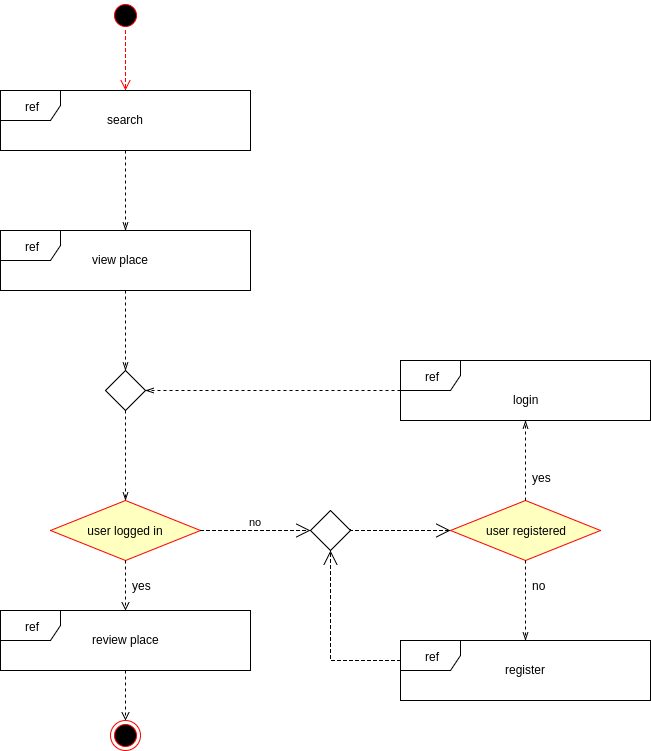
\includegraphics[width=15cm]{interactionDiagram.png}
\caption{interaction overview diagram}
\end{figure}



\subsection{REST API module}
This is a sort of a wrapper for OPR App that provides a REST API interface, to be used by the mobile app.
\\For the REST API Module, I worked using the backwards approach; I started by writing the documentation of the functionalities first.\\



The services provided by the API are:
\begin{itemize}

\item Login
\item Register
\item Logout
\item Search for places
\item Get place details
\item Get reviews
\item Add review
\end{itemize}
The functions that require the transfer of critical data were designed to use the HTTP POST
method because it’s more secure and it is the standard for this type of operations, for instance
we used POST for the authentication and registration functions. We also chose HTTP POST for
posting reviews, because it contains the authentication token, which is critical data, and it
contains the review’s text, whose size might exceed the GET data size limit.\\
As for the other functionalities we used HTTP GET methods. One of the benefits of using GET
here is that you can share and bookmark links easier when the data is included in the URL.

\paragraph{Login}~\\
Authenticate the user with the system and obtain the auth\_token

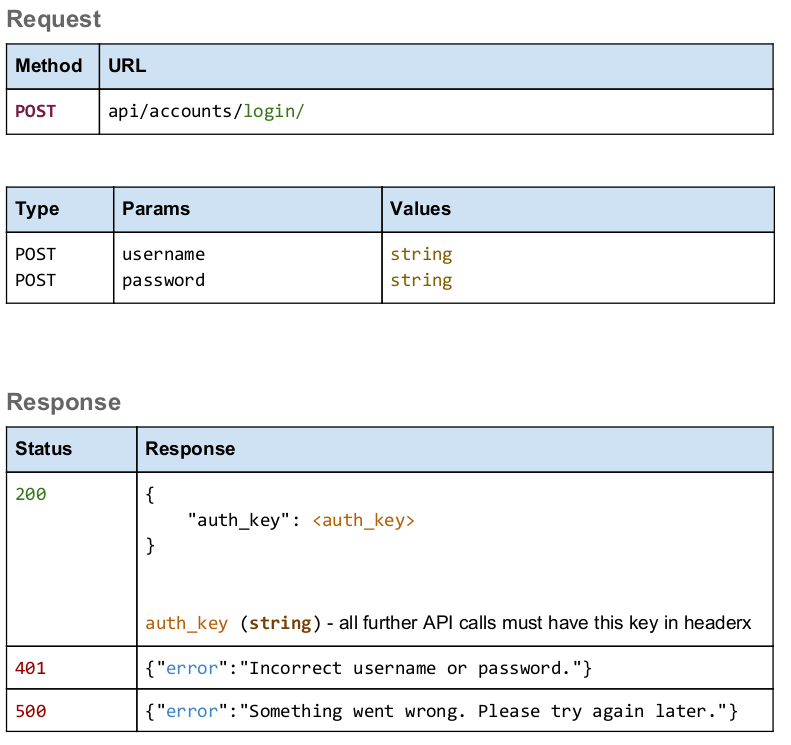
\includegraphics[width=15cm]{loginDoc.png}


\paragraph{Register}~\\
Create and add a new user to the app

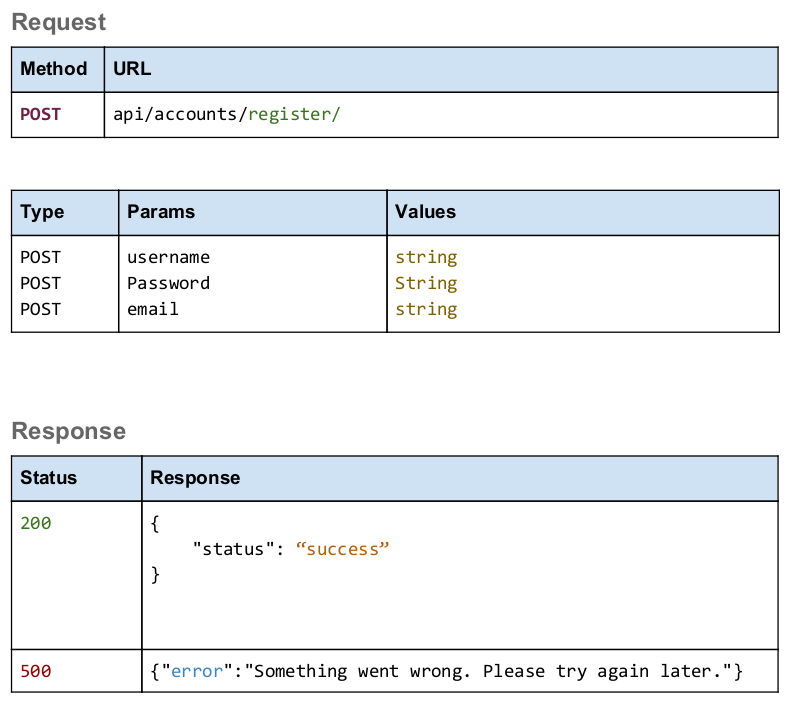
\includegraphics[width=15cm]{registerDoc.png}


\paragraph{Logout}~\\
Log out the current user

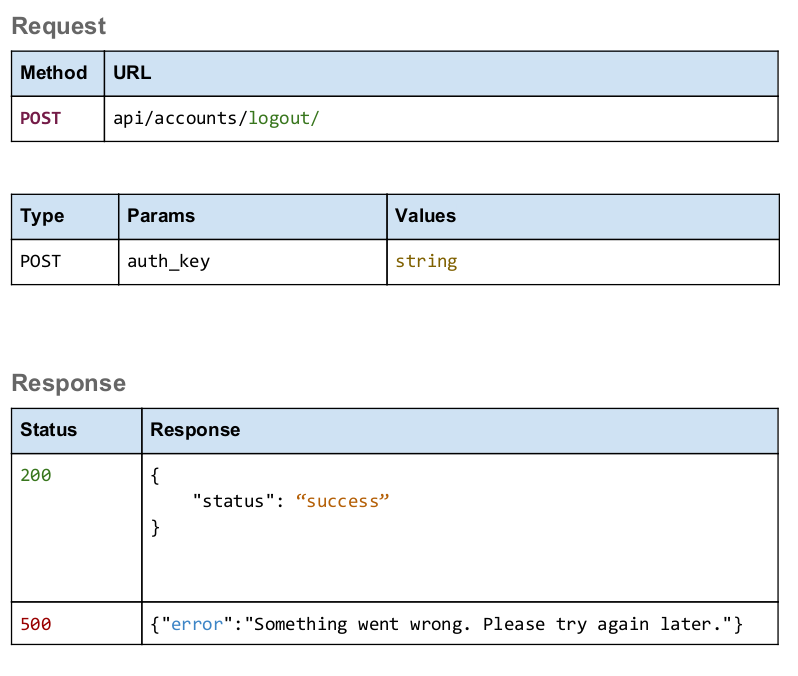
\includegraphics[width=15cm]{logoutDoc.png}


\paragraph{Search for places}~\\
Search for hotels, restaurants or activities

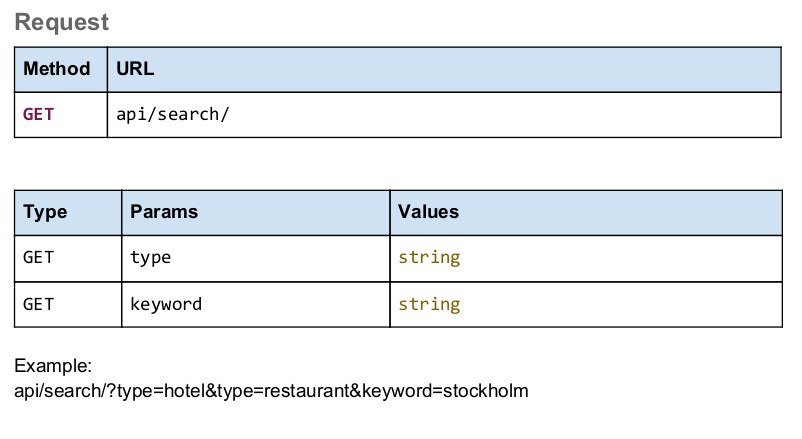
\includegraphics[width=15cm]{searchDoc.png}

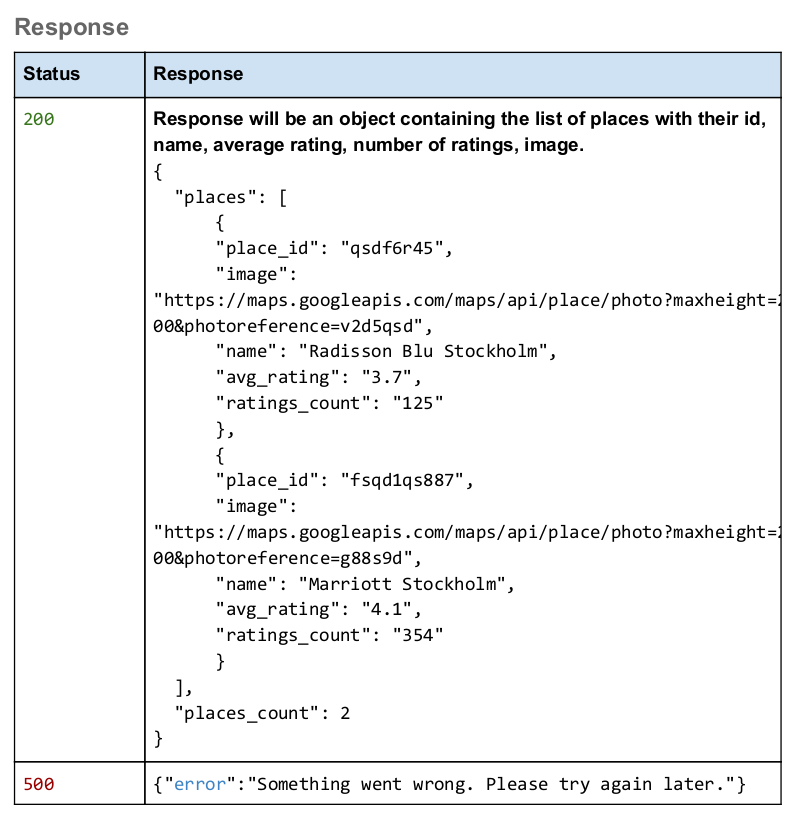
\includegraphics[width=15cm]{searchDocResponse.png}



\paragraph{Get place details}~\\
Get the the details of a specific place using it’s place\_id

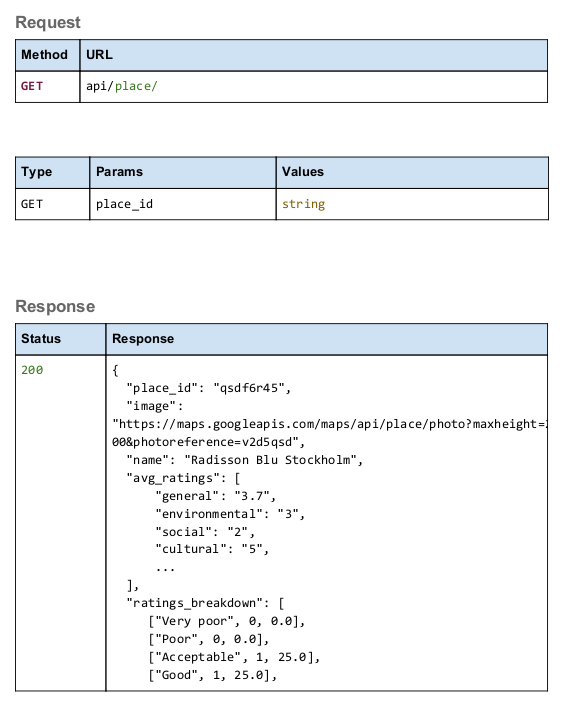
\includegraphics[width=15cm]{detailsDoc.png}

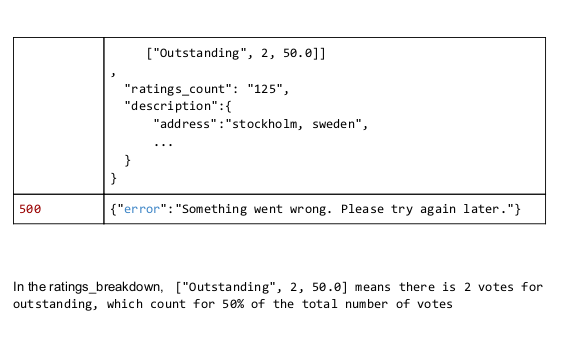
\includegraphics[width=15cm]{detailsDocResponse.png}

In the ratings\_breakdown, ​ ["Outstanding", 2, 50.0] means there is 2 votes for
outstanding, which count for 50% of the total number of votes

\paragraph{Get reviews}~\\
Get the reviews of a place using it’s place\_id

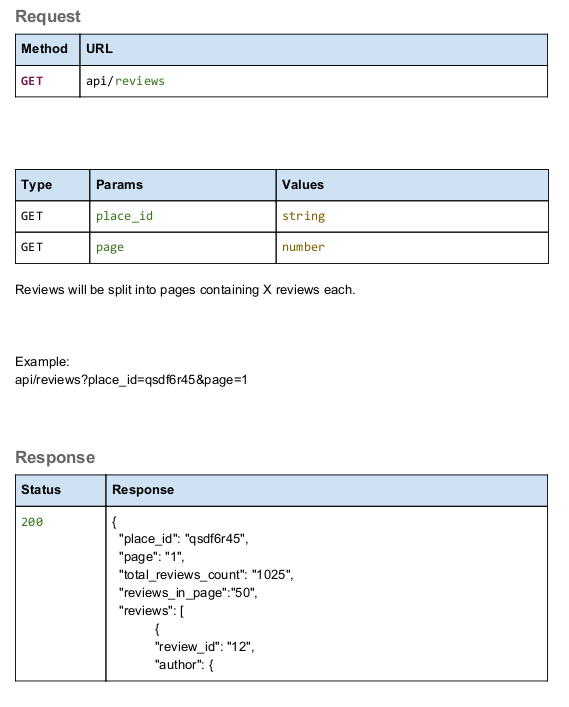
\includegraphics[width=15cm]{reviewsDoc.png}

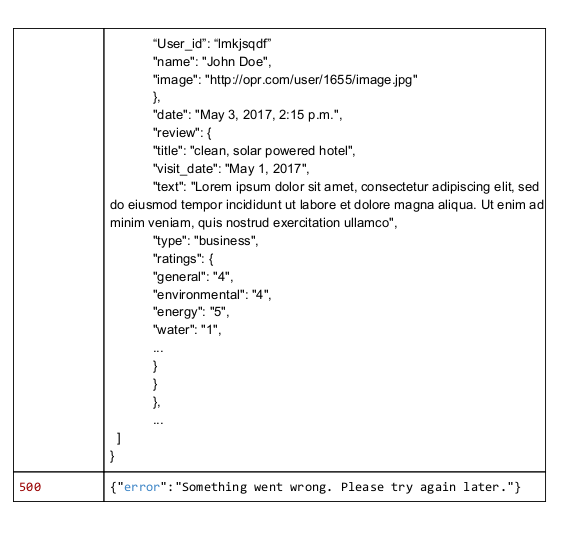
\includegraphics[width=15cm]{reviewsDocResponse.png}


\paragraph{Add review}~\\
Add a new review to a place

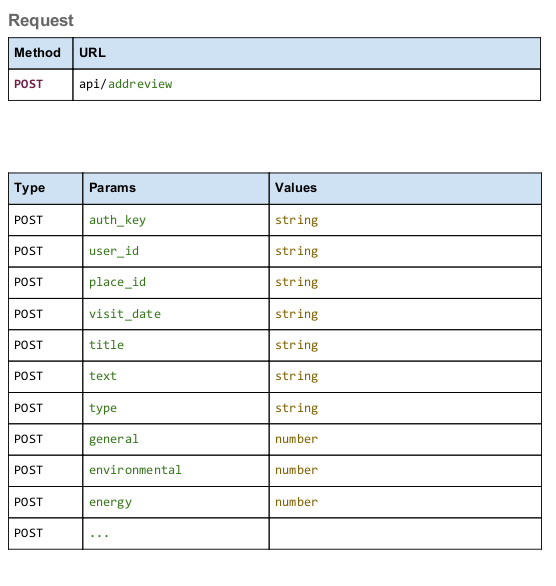
\includegraphics[width=15cm]{addDoc.png}

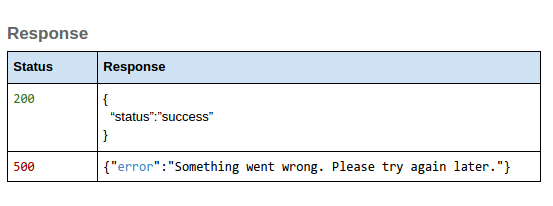
\includegraphics[width=15cm]{addDocResponse.png}


\chapter{Implementation}
\section{Technology choices}

\paragraph{Frontend}~\\
For the front-end I used HTML/CSS/JS with JQuery library because it facilitates basic
functionalities like DOM manipulation.\\
I also used twitter’s Bootstrap in order to use it’s prebuilt components like the buttons.
The app is responsive but has some responsiveness-bugs; I didn’t fix these because of time
constraints and because the front-end is being redesigned by a professional designer anyway.

\paragraph{Backend}~\\

The programming language used is Python, with the framework Django.\\
After careful thought I went with this choice because of several factors, including but not limited
to:
\begin{itemize}

\item Portability: this stack is cross-platform and can run on linux as well as windows
\item  Lots of tools out of the box: this choice offers:
\begin{itemize}

\item Runtime + Web framework
\item Package manager (PIP)
\item A database to test with (sqlite)
\item A lightweight development server
\item Unit testing library
\end{itemize}
\item Integrated ORM
\item Lots of libraries and ready-to-use components
\item  Abundant support and documentation
\item  Stability and reliability
\item  Scalability
\item  Great community
\end{itemize}

This boils down to creating a prototype quickly with this technology stack; we can get a lot done
in little time. Timing is a crucial part of this project, especially in this phase (prototyping).


\paragraph{Database}~\\

While comparing multiple databases, I ended up with two of the most popular databases to
compare between: MySQL and PostgreSQL.\\
The following table shows some differences of how things work in MySQL vs. in PostgreSQL.


\begin{table}[H]
\centering
\begin{tabular}{|l|l|l|}
\hline
                  & MySQL                                                                                                            & PostgreSQL                                                                                                                                                                                                      \\ \hline
CREATE INDEX      & \begin{tabular}[c]{@{}l@{}}Entire table is locked for\\ writes\end{tabular}                                      & \begin{tabular}[c]{@{}l@{}}Entire table is locked for\\ writes.But PSQL has \\“CREATE INDEX\\ CONCURRENTLY”\\that permits the creation of\\ index without locking the\\ entire table (but it’s slower)\end{tabular} \\ \hline
Adding new column & \begin{tabular}[c]{@{}l@{}}Entire table data needs to be\\ rewritten\end{tabular}                                & Instantaneous                                                                                                                                                                                                   \\ \hline
Connection model  & \begin{tabular}[c]{@{}l@{}}One thread/connection:\\ Easy to create but hard to\\ monitor and manage\end{tabular} & \begin{tabular}[c]{@{}l@{}}One process/connection:\\ Easier to monitor and\\ manage\end{tabular}                                                                                                                \\ \hline
\end{tabular}
\caption{MySQL vs PostgreSQL}
\label{my-label}
\end{table}

I decided to use PostgreSQL as a database because of the previous comparison and because
it’s well supported by Django.\\
This choice is in someway influenced by the previous choice.

\paragraph{Server}~\\

I used an Ubuntu 16.04 LTS Virtual Private Server for hosting the project.
Ubuntu has a great community and support, is reliable, and the Long Term Support (LTS)
version remains maintained for 5 years, so we won’t have to worry about upgrading the system
for five years.\\
Ubuntu is based on Debian, which is one of the most stable Linux distributions ever.\\
The provider of the VPS is Amazon Web Service (AWS). I used AWS because it offers a free
tier during the first year of use, and because it has extensive capabilities beyond offering a
simple VPS. One of the capabilities that interested me the most is the ease of scaling and
setting up load balancers for the project.

\paragraph{Web Server}~\\
I had the choice between Apache HTTP Server and NGINX.\\
Both of them are great web servers and have great communities and support, and both of them
are open source as well.\\
I went with NGINX because it’s better performance-wise and is taking over Apache.

\begin{figure}[H]
\centering
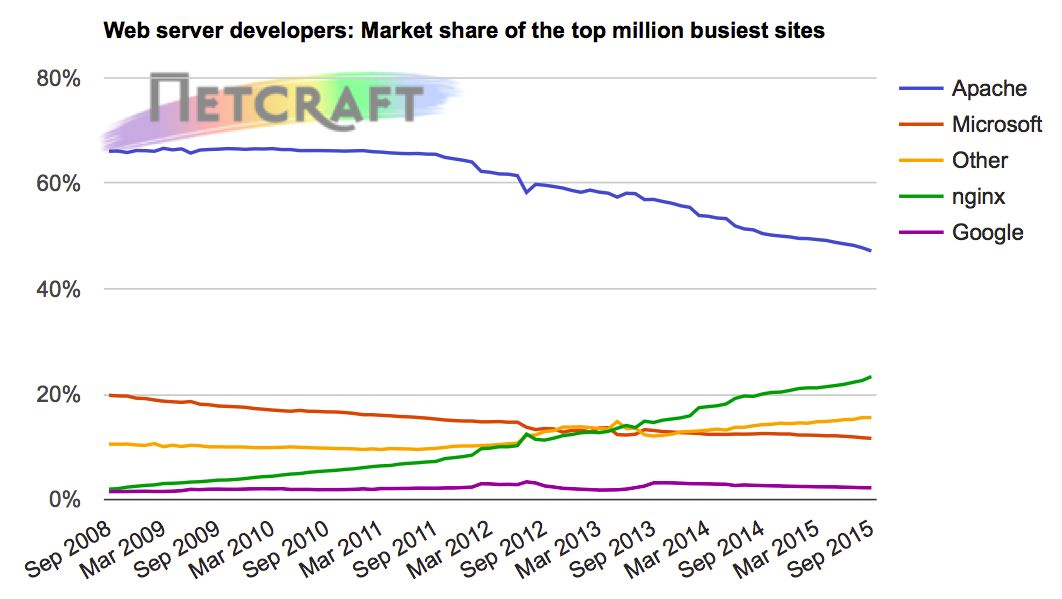
\includegraphics[width=15cm]{apache.png}
\caption{Chart showing how nginx’s user base is growing while apache’s is regressing}
\end{figure}

\paragraph{Python Application server}~\\
I used Gunicorn as application server because it is the most popular and the best supported
server.
\paragraph{Additional Frameworks/libraries}

\subparagraph{Django-rest-framework}~\\
Django-rest-framework (DRF) supports the creation of REST APIs on top of Django.
This framework is django’s standard tool to create REST APIs.

\subparagraph{Django-allauth}~\\
This is a library addressing authentication, registration, account management and social
authentication



\subparagraph{Django-rest-auth}~\\
This library makes the previously mentioned library (allauth) accessible via REST API




\subparagraph{Django-review}~\\
This is a library facilitating the creation of reviews and ratings. I found multiple libraries offering
reviews-related functionalities. I chose this library because it’s kept updated and is backed by a
company.

\section{Screenshots}
\subsection{Web interface}

\begin{figure}[H]
\centering
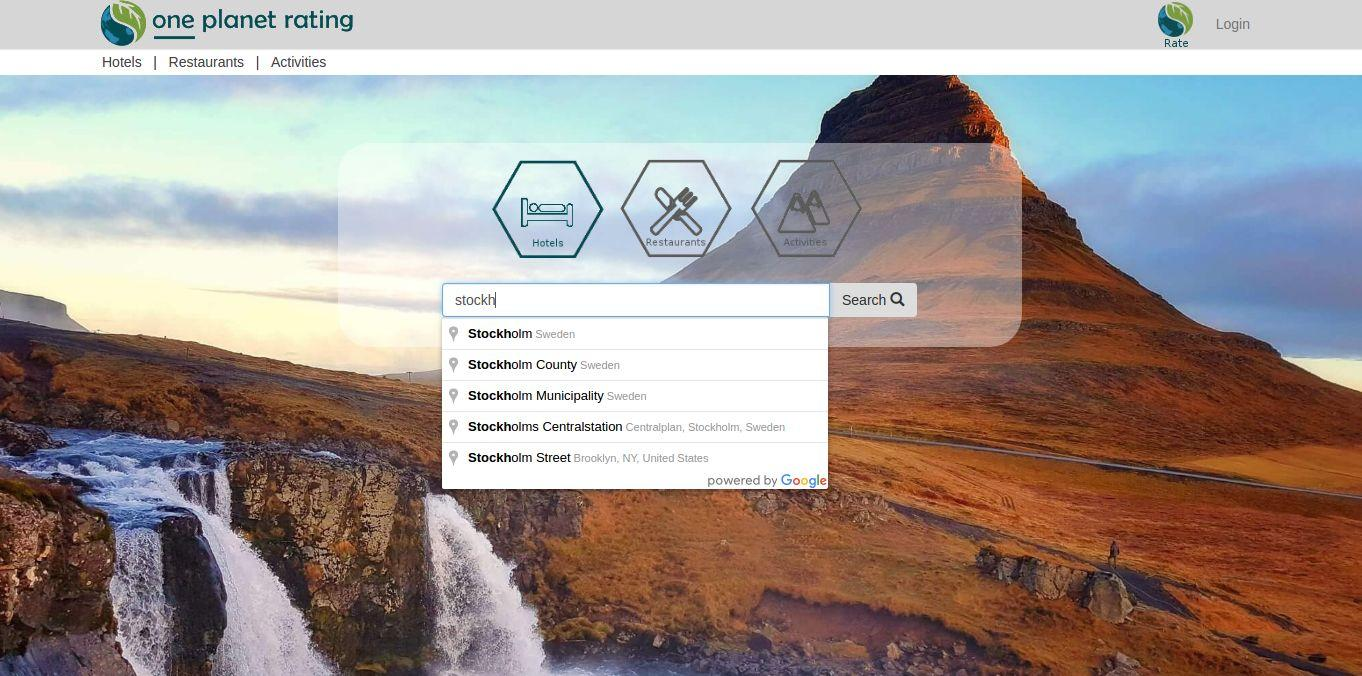
\includegraphics[width=15cm]{landing.jpg}
\caption{the landing screen of the app}
\end{figure}

When first accessed, the app shows the previous landing page. From there the user is able to
search for a place using the search bar.\\
The user is also to access the login screen from there.\\
Other functionalities include listing the popular and trending hotels using the links in the top left
corner, but these functionalities haven’t been implemented yet.



\begin{figure}[H]
\centering
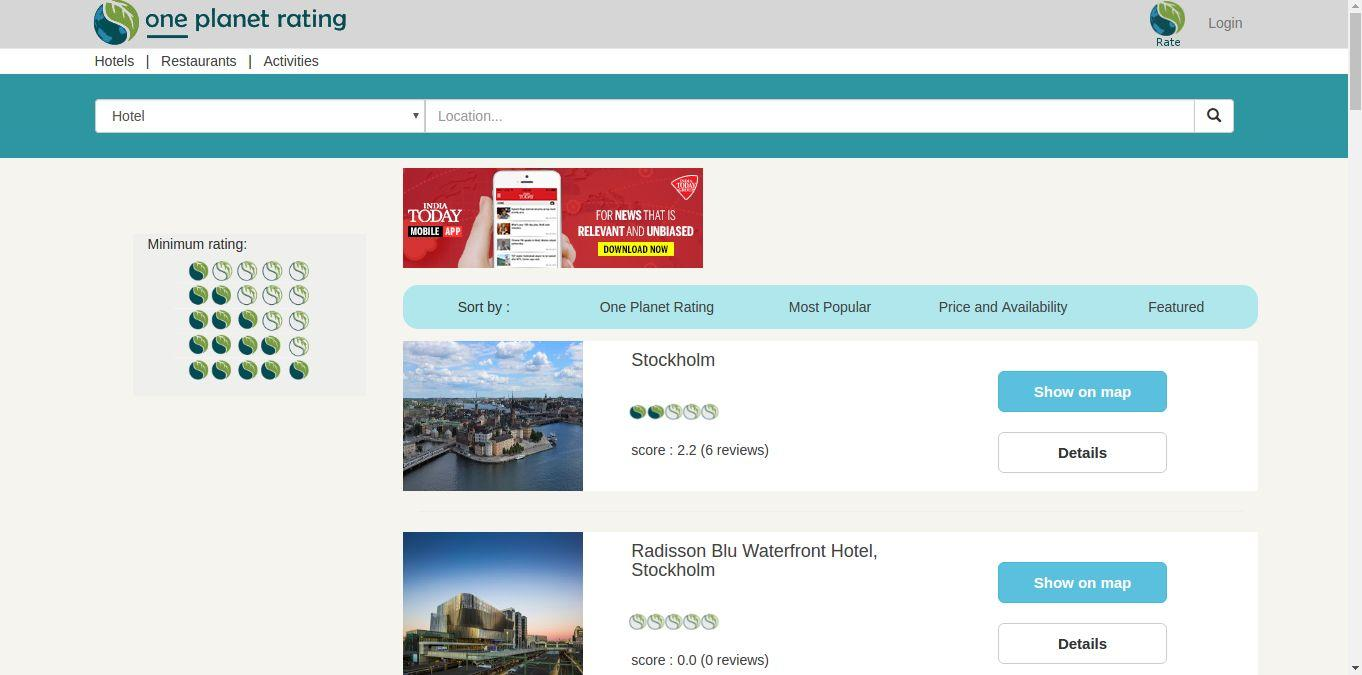
\includegraphics[width=15cm]{search.jpg}
\caption{search screen}
\end{figure}

After the landing page, when a user searches for a place he will get redirected to this search
screen which includes the results retrieved from Google’s places service. The search results
include the name and the picture (from google) as well as the number of reviews and the
average score from the reviews posted on OPR.




\begin{figure}[H]
\centering
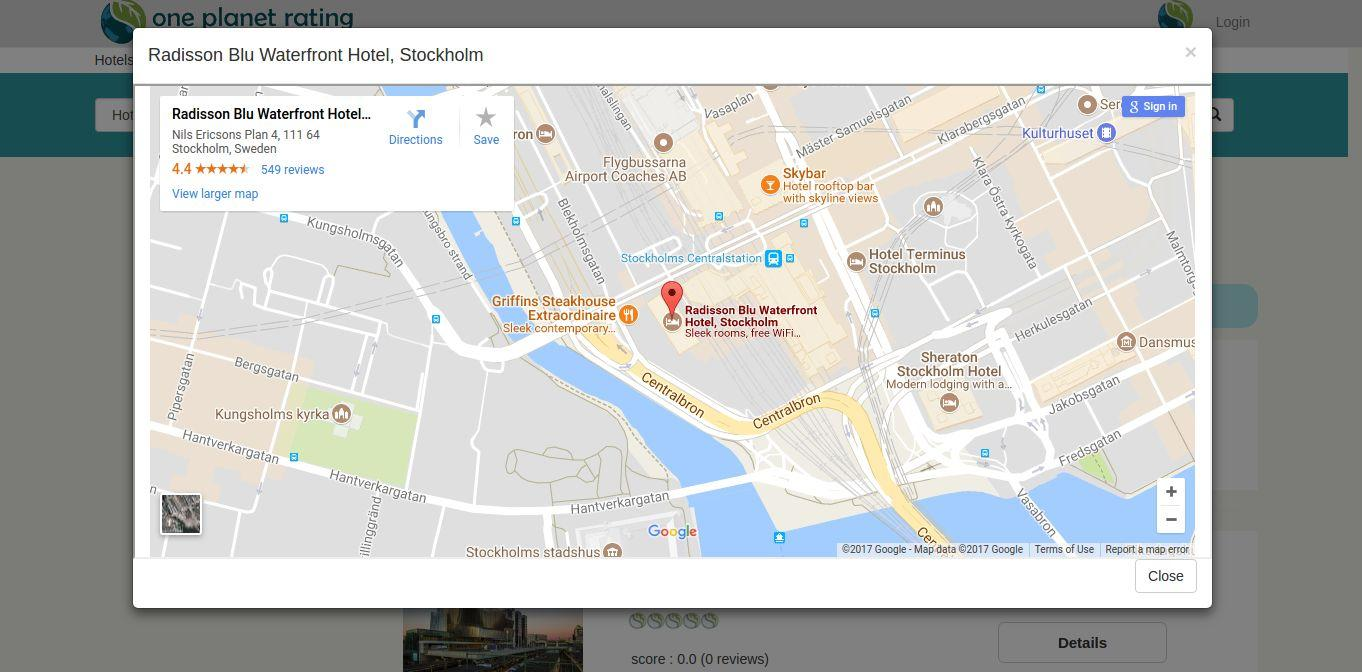
\includegraphics[width=15cm]{map.jpg}
\caption{showing the location of a place on the map}
\end{figure}

From the search screen, the user is able to click the “show on map” button to see the selected
place on Google maps. The map is shown in a modal view in order for the user not to quit
OPR’s site.




\begin{figure}[H]
\centering
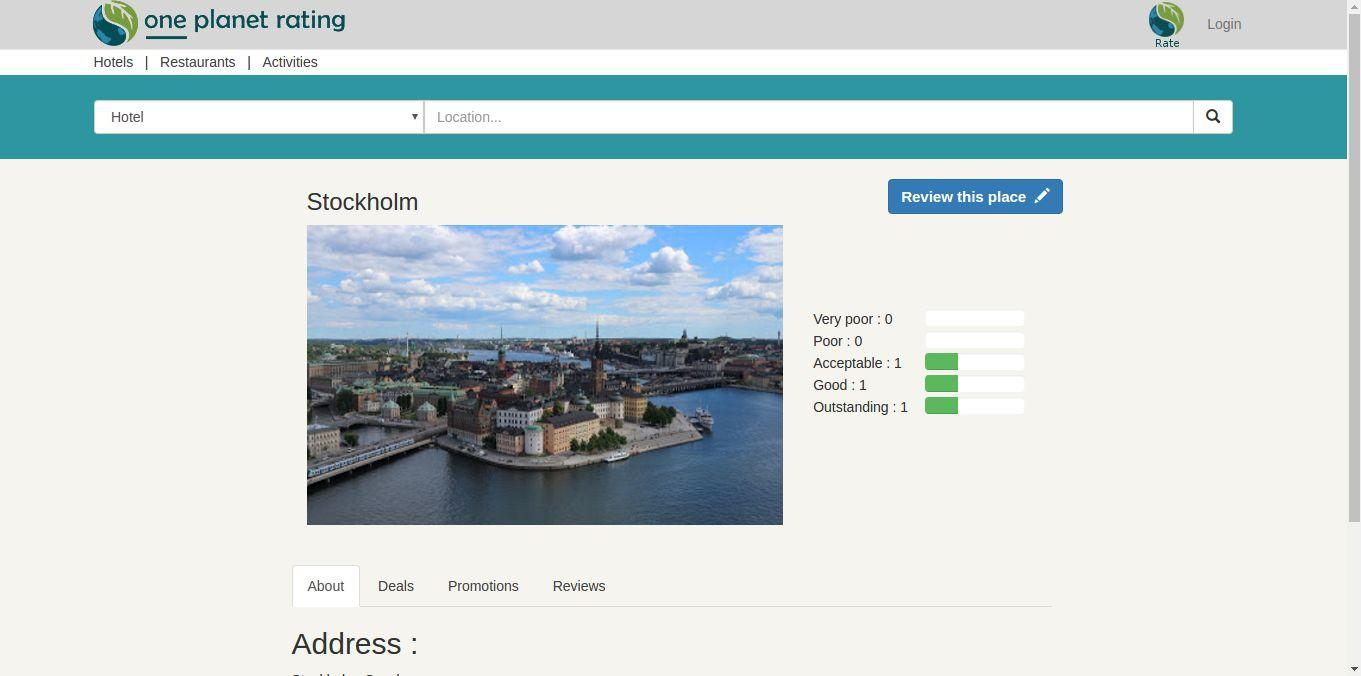
\includegraphics[width=15cm]{details.jpg}
\caption{place details}
\end{figure}

When the user selects a place to see its details, he’s shown this screen; it contains the name,
picture and basic details of the place. This same screen also contains the reviews and a chart
showing the numbers and proportions of ratings.





\begin{figure}[H]
\centering
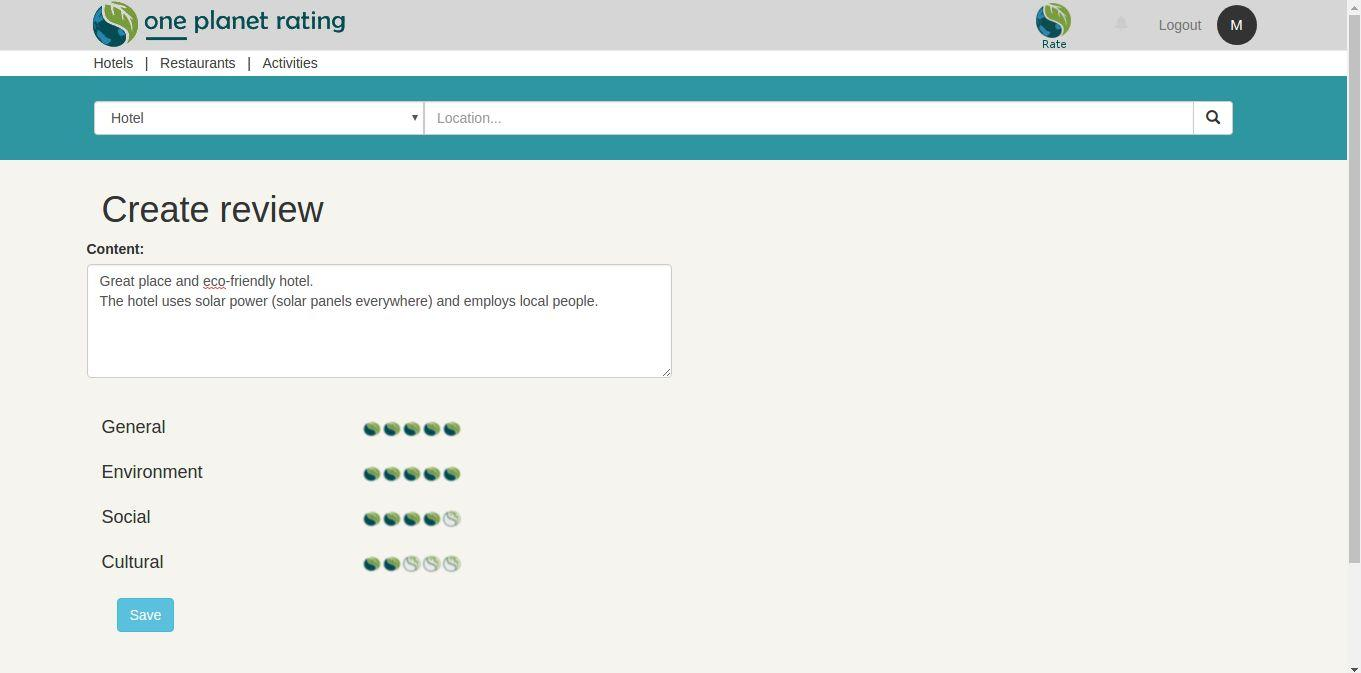
\includegraphics[width=15cm]{createReview.jpg}
\caption{Creating a review}
\end{figure}


When the user chooses to create a review, the app first checks whether he’s logged in.\\
If not, the user is redirected to the login screen, otherwise this form appears. The form allows
the user to enter a text review as well as ratings following specific criteria.




\begin{figure}[H]
\centering
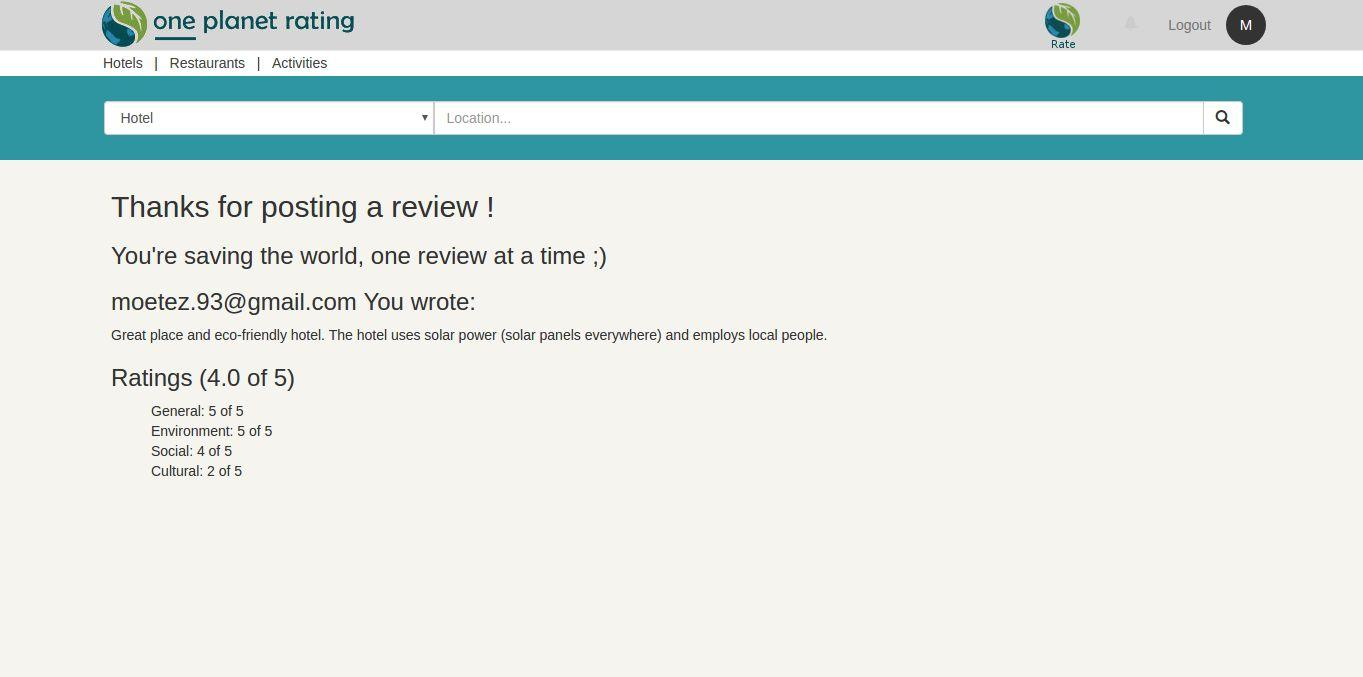
\includegraphics[width=15cm]{thanks.jpg}
\caption{Thanks screen}
\end{figure}

After a member posts a review successfully, he’s shown a thanks screen.




\begin{figure}[H]
\centering
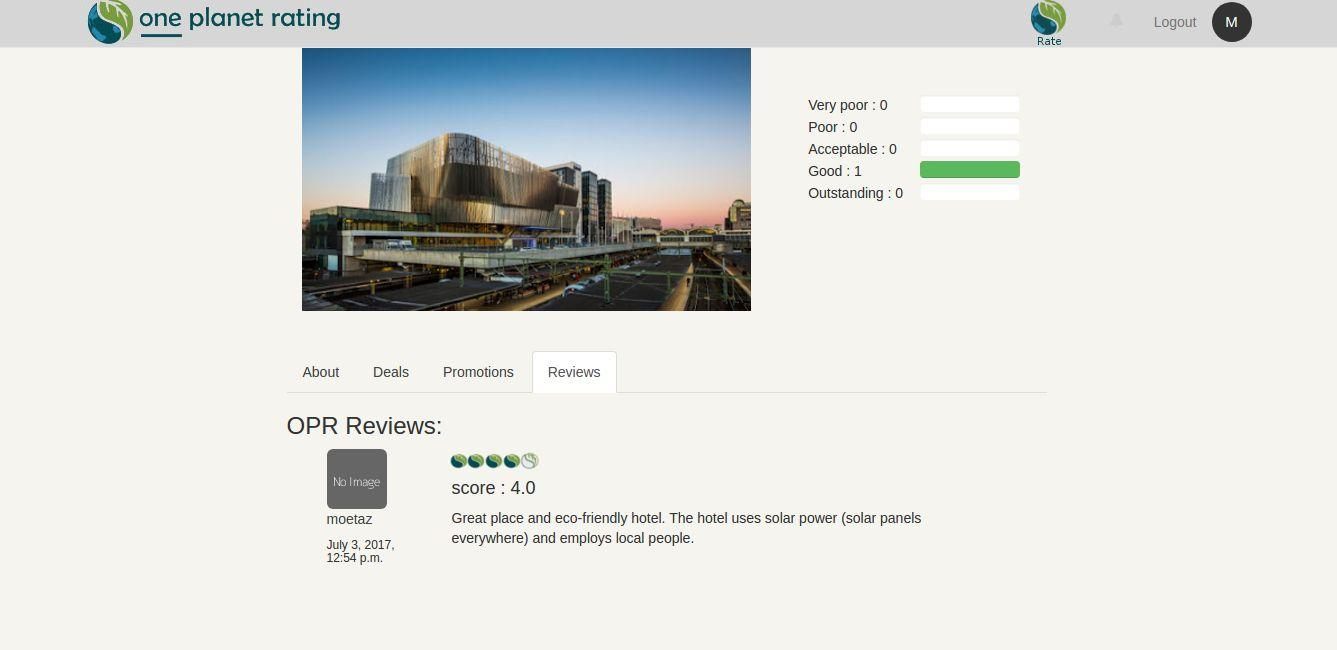
\includegraphics[width=15cm]{review.jpg}
\caption{Showing a review}
\end{figure}

After a review is added, it is displayed as in this screenshot. The score, text, username and date
are currently shown. Other features are being added like the user’s photo and the categorized
ratings.

\subsection{API}



\begin{figure}[H]
\centering
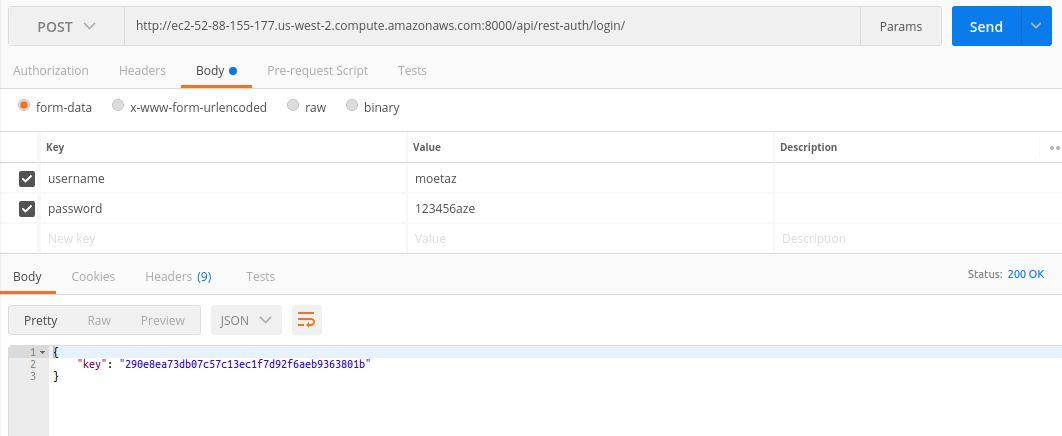
\includegraphics[width=15cm]{apilogin.jpg}
\caption{API Login}
\end{figure}

This screenshot shows an example of a login request through the REST API.



\begin{figure}[H]
\centering
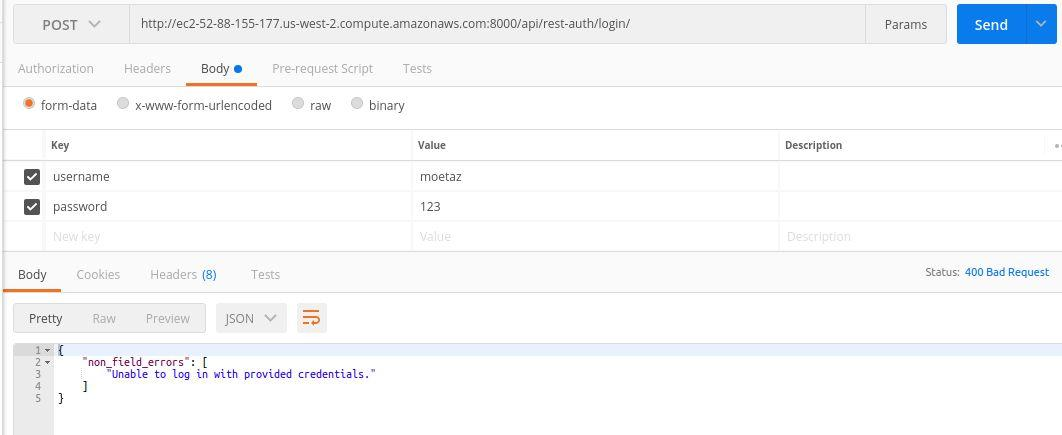
\includegraphics[width=15cm]{apiloginfail.jpg}
\caption{API Login failure}
\end{figure}

In case of failure (wrong credentials), an error message is sent back to the user.





\begin{figure}[H]
\centering
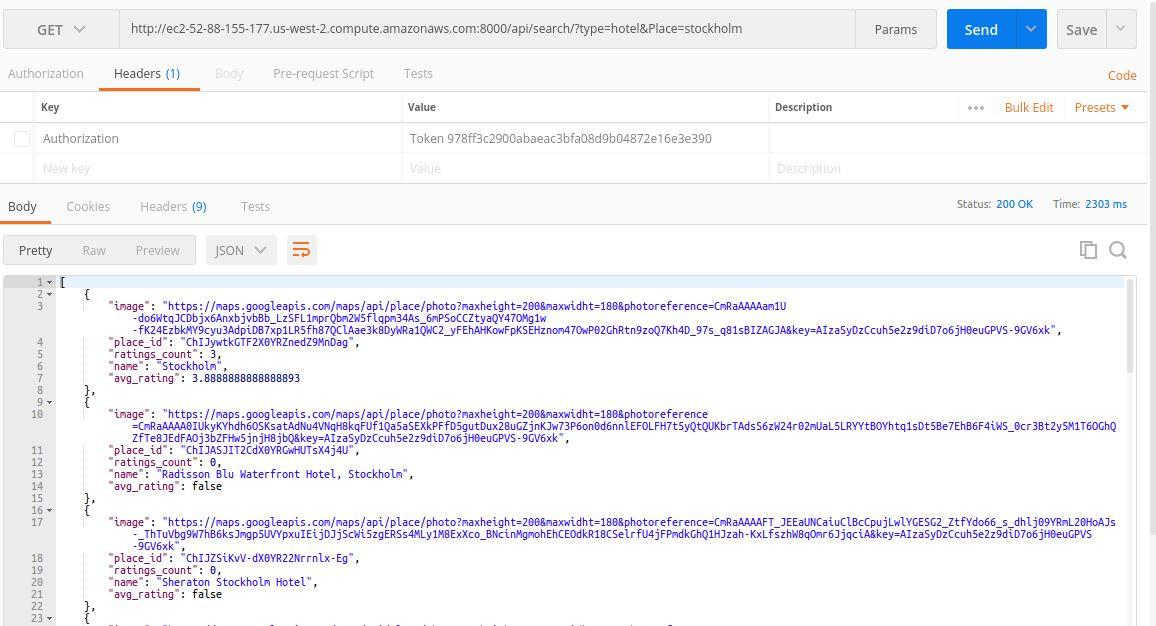
\includegraphics[width=15cm]{apisearch.jpg}
\caption{API search request}
\end{figure}

This screenshot shows the response to a search query. The query includes as parameters the
type of place (hotel, restaurant..) as well as a keyword to specify the location.\\
The response contains the name, image, place\_id, ratings count , and the average rating.\\
The name and image are displayed as is. The ratings count and the average rating, however,
are used to display the globes/stars next to each place in the results list. The place\_id is used to
get the place’s map or the place’s details.






\begin{figure}[H]
\centering
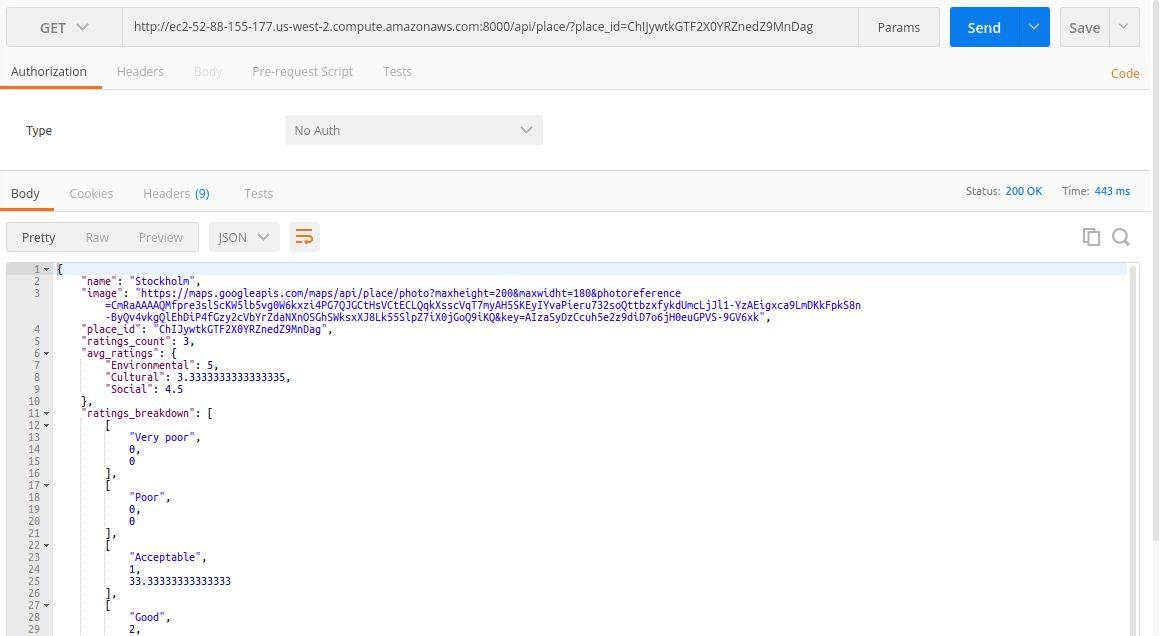
\includegraphics[width=15cm]{apidetails.jpg}
\caption{API search request}
\end{figure}

When requesting the details of a place, the request includes the place\_id of the place.\\
Obviously the response includes the name and image of the place, it also includes the number
and averages of ratings. It also contains the ratings breakdown, which consists of the
proportions of the ratings arranged by the number of stars ( 0 star = very poor, 1 star = poor...)





\begin{figure}[H]
\centering
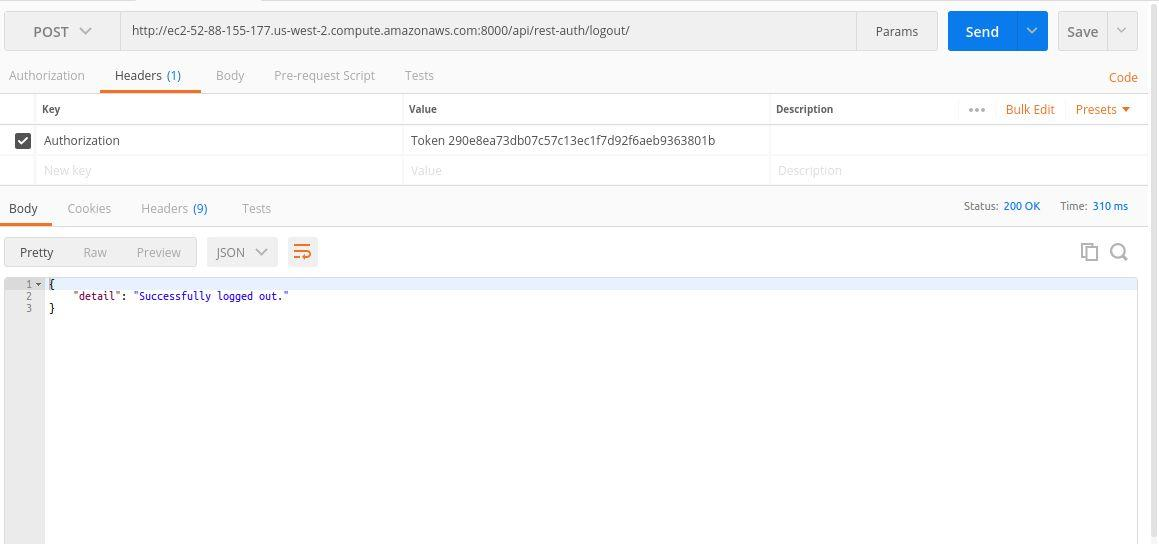
\includegraphics[width=15cm]{apilogout.jpg}
\caption{Logout API call}
\end{figure}

This screenshot shows a successful logout call. The authentication is based on an authorization
token stored in the DB. After logging out, that token is deleted.

\section{Deployment}

\paragraph{AWS EC2 Security setup}~\\



\begin{figure}[H]
\centering
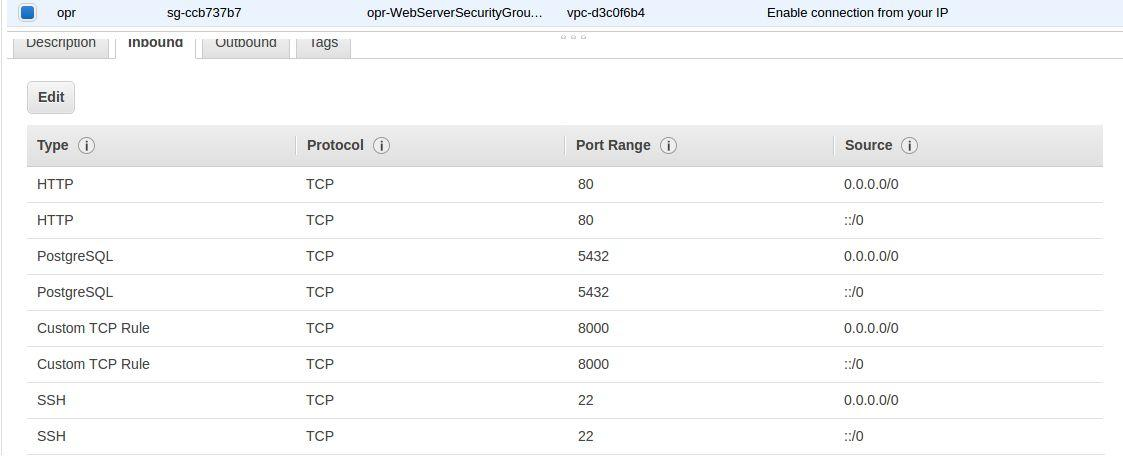
\includegraphics[width=15cm]{ec21.jpg}
\caption{AWS EC2 allowed inbound traffic}
\end{figure}


\begin{figure}[H]
\centering
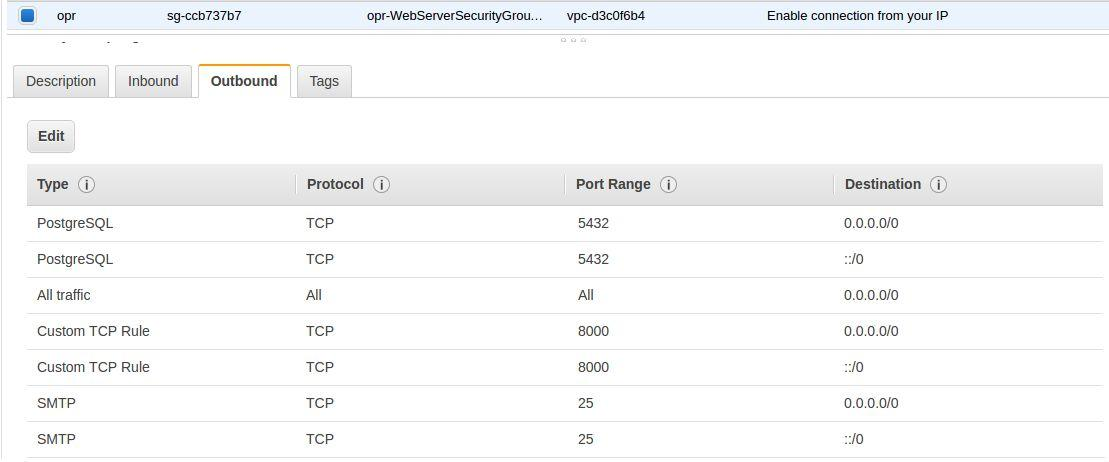
\includegraphics[width=15cm]{ec22.jpg}
\caption{AWS EC2 allowed outbound traffic}
\end{figure}

A problem I encountered during the deployment is to get the server to reply for requests.
In the beginning I was even unable to ssh into the VPS. It turned out, for security reasons AWS
blocks all incoming and outcoming traffic.


\paragraph{AWS RDS setup}~\\


\begin{figure}[H]
\centering
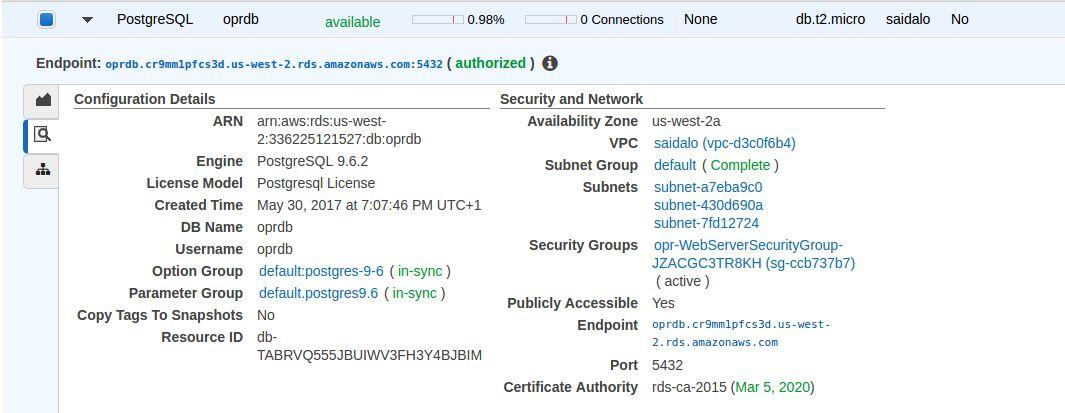
\includegraphics[width=15cm]{rds.jpg}
\caption{AWS RDS setup}
\end{figure}

I used AWS RDS for hosting the database because security wise it’s better approach to host the
database separately from the app. Another advantage of AWS RDS is that it automatically
creates backups of the DB.\\
First I hosted a local db for testing purposes then I moved the same DB to RDS.


\paragraph{NGINX setup}~\\



\begin{figure}[H]
\centering
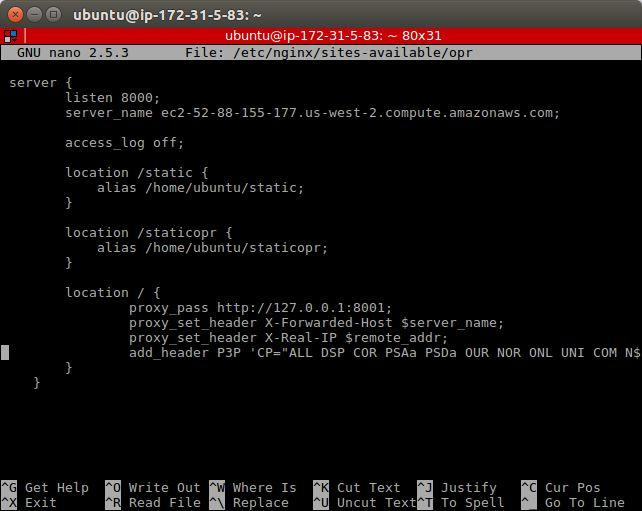
\includegraphics[width=15cm]{nginx.jpg}
\caption{NGINX setup}
\end{figure}

NGINX is the entrypoint to the app. It’s also the web server used to serve the app. NGINX was
setup to listen on port 8000 and to serve the static files like the images and css ( practically
every url pointing to /static). In case of non static files, NGINX redirects the request to gunicorn
which is the python server that’s serving the app.

\section{Testing}

For the development of searchAd module, which is a sort of standalone library, I also created
unit tests for it.\\
The unit tests ensure that the code works correctly, and helps verify that the code didn’t break
after some changes. This provides better quality and saves more time.


\begin{figure}[H]
\centering
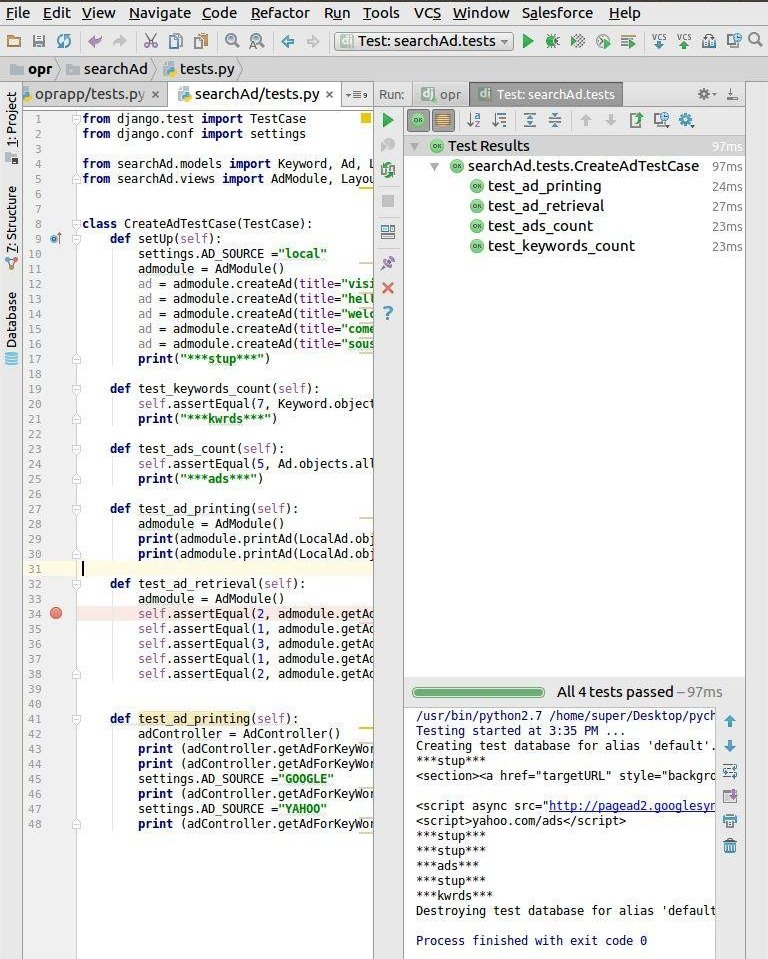
\includegraphics[width=15cm]{unittests.jpg}
\caption{unit tests}
\end{figure}


I also tested the performance of the app (load speed) using google’s Pagespeed Insights, and I
got some amazing results:




\begin{figure}[H]
\centering
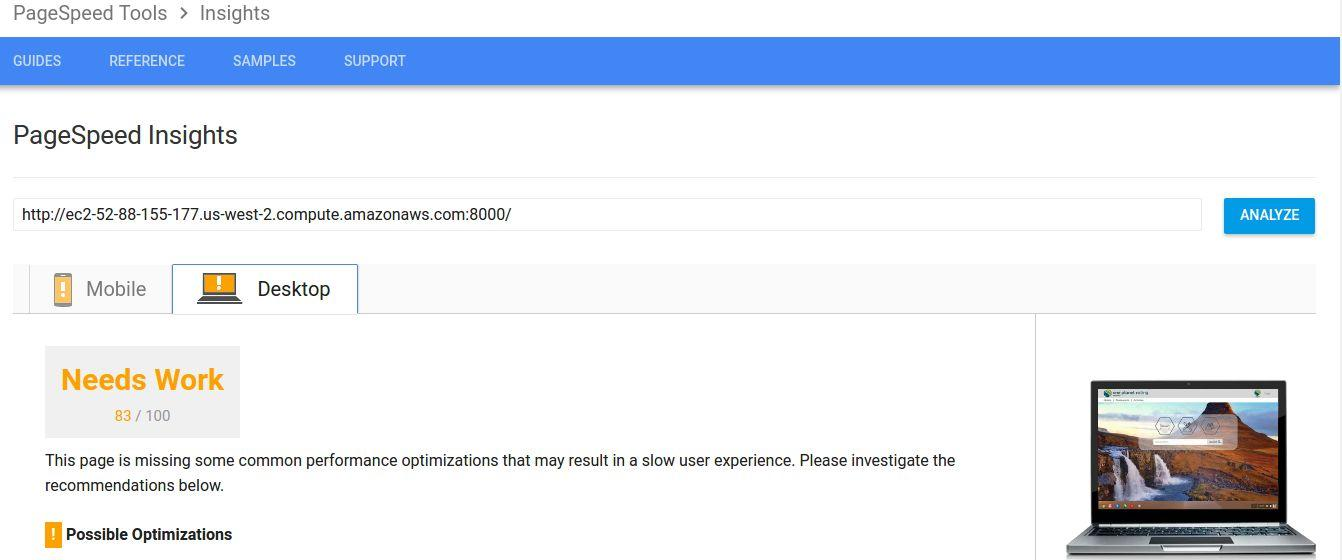
\includegraphics[width=15cm]{speed1.jpg}
\caption{landing page speed test}
\end{figure}



\begin{figure}[H]
\centering
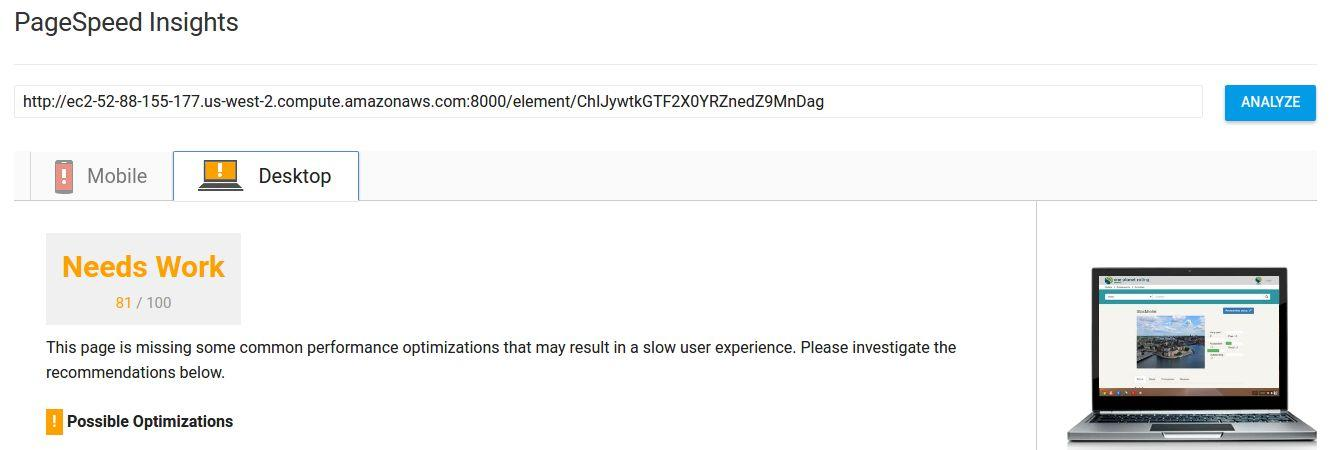
\includegraphics[width=15cm]{speed2.jpg}
\caption{details page speed test}
\end{figure}

Below is included the result for the same test applied to facebook.com for comparison purposes:




\begin{figure}[H]
\centering
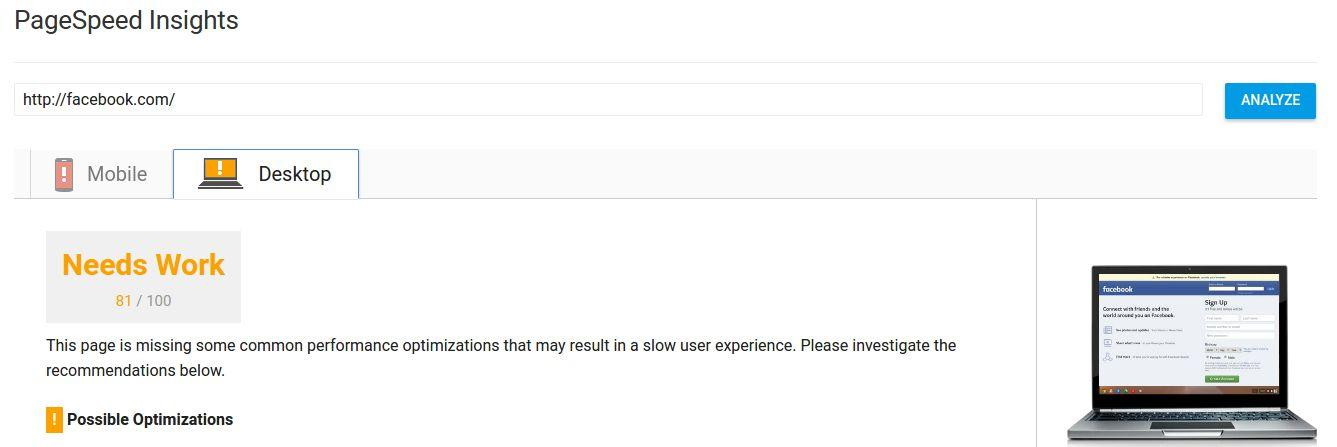
\includegraphics[width=15cm]{fbtest.jpg}
\caption{facebook page speed test}
\end{figure}


I also tested the performance of the app using blazemeter. I tested the service with 50
simultaneous virtual users and the results were good.




\begin{figure}[H]
\centering
\includegraphics[width=15cm]{blaze.jpg}
\caption{concurrent users test}
\end{figure}

With 50 simultaneous users the response time was ~170ms which is okay. Note that the
performance is influenced by the performance amazon’s server, which is very limited but easily
scalable. For the development, I went with a low-performance server instance because of
budgetary reasons, but we can scale up easily later when we need to.
The used instance is an AWS EC2 t2.micro with the following specs:
\begin{itemize}
\item RAM: 1 GB
\item vCPUs: 1
\end{itemize}

\section{Work environment}
All of the development was made on my personal laptop which has the following specs:
\begin{itemize}
\item RAM: 8GB
\item CPU: Intel core i7
\item OS: Ubuntu 16.04 LTS
\end{itemize}

During the development I used the IDE PyCharm.
For version control we used Git, hosted on BitBucket.
Communication was all held on Slack.
The diagrams were made using Dia and draw.io
~\\~\\
In the beginning of the project I also did some graphic design using GIMP, which is an open
source and free alternative to photoshop.
I also used InvisionApp to create an interactive prototype using the mockups I designed.
Chrome developer tools were used extensively for debugging and tweaking the frontend.
Postman was used to test the REST requests for the API.
Python’s unittest was used for the unit tests.

%
%\section{Etat de l'art}
%
%Morbi pharetra posuere sem eget pharetra. Phasellus commodo purus
%ac eros consequat a sodales orci sodales. In vitae augue vel nisl
%tincidunt elementum ac eu lorem. Nam placerat sapien quis lorem facilisis
%molestie.
%
%
%\subsection{Exemple site 1}
%
%Cras pretium, sapien ac interdum suscipit, arcu ante ultricies quam,
%eu vulputate nisl odio vitae tellus. In eget odio tellus, non varius
%dolor. Cras porttitor convallis augue, at viverra tortor faucibus
%id. Donec sagittis tristique est, a bibendum quam rutrum at. Vestibulum
%ac mi ante, eu facilisis ligula. Ut nec feugiat ipsum. Vivamus elementum
%dolor ut ligula pharetra ac convallis lacus fermentum. Phasellus suscipit
%lacus vel odio tristique sed ultricies elit varius. Phasellus elit
%nisi, pellentesque sit amet rhoncus non, aliquet interdum lorem. Nullam
%et neque nibh, non mattis nulla. Nam sit amet tincidunt arcu. Aliquam
%consequat laoreet quam, vitae mattis nunc gravida eget. Proin nec
%massa tortor, ut sagittis odio. Donec bibendum ipsum sed nibh ornare
%gravida. Donec volutpat felis nec massa posuere fermentum. Donec tincidunt
%faucibus velit non semper (voir figure \ref{fig:mon_image}). 
%
%\begin{figure}[H]
%\noindent \begin{centering}
%%\includegraphics{frog.jpg}
%\par\end{centering}
%
%\caption{\label{fig:mon_image}Mon image du premier site avec référence}
%\end{figure}
%
%
%Nam eu leo justo. Praesent accumsan consequat tellus, et hendrerit
%magna ornare ut. Nullam ac orci ac magna ullamcorper tristique. Cras
%lacus augue, congue in ullamcorper id, cursus sit amet odio. Fusce
%dui ligula, vehicula ut pharetra sit amet, feugiat ac arcu. Mauris
%interdum pretium urna a posuere. Fusce in porttitor ante. Suspendisse
%potenti. Cras mattis adipiscing enim. Duis varius, neque in posuere
%porttitor, odio urna bibendum nunc, sit amet laoreet sem orci id lorem.
%Ut ultrices mauris quis purus fringilla tristique. Aliquam non nunc
%nulla, vitae sagittis nibh. Mauris in diam felis. Cras quis neque
%sed turpis condimentum porta ac a purus. Duis posuere pellentesque
%feugiat. Nunc tempus, ligula ac scelerisque dignissim, neque mauris
%venenatis lorem, nec consectetur sem odio in tortor. Sed velit tellus,
%egestas ut malesuada nec, interdum a eros. Class aptent taciti sociosqu
%ad litora torquent per conubia nostra, per inceptos himenaeos. 
%
%\begin{table}[H]
%\noindent \begin{centering}
%\begin{tabular}{|c|c|c|}
%\hline 
%A & B & C\tabularnewline
%\hline 
%\hline 
%X & Y & Z\tabularnewline
%\hline 
%\end{tabular}
%\par\end{centering}
%
%\caption{Un exemple de tableau}
%
%
%\end{table}
%
%
%Nulla tellus augue, mattis sed scelerisque id, aliquet sit amet nunc.
%Nullam nulla metus, volutpat vitae tempus vel, rhoncus id elit. Quisque
%non semper urna. Cras molestie mollis sapien egestas rutrum. Proin
%tincidunt laoreet est id fringilla. Aliquam vel risus augue. Mauris
%scelerisque tortor arcu, sed auctor tellus. Donec egestas luctus varius.
%Vestibulum tortor erat, elementum sollicitudin tempus quis, tempus
%nec magna. Sed sed metus turpis, in pulvinar orci. 
%
%Sed sed augue vel velit interdum bibendum. Donec imperdiet interdum
%elit eu elementum. Vivamus pulvinar pharetra erat, et mattis est iaculis
%a. Pellentesque eu nunc sit amet orci ultrices tempus vitae non massa.
%Morbi pharetra posuere sem eget pharetra. Phasellus commodo purus
%ac eros consequat a sodales orci sodales. In vitae augue vel nisl
%tincidunt elementum ac eu lorem. Nam placerat sapien quis lorem facilisis
%molestie. 
%
%
%\subsection{Exemple site 2}
%
%Cras pretium, sapien ac interdum suscipit, arcu ante ultricies quam,
%eu vulputate nisl odio vitae tellus. In eget odio tellus, non varius
%dolor. Cras porttitor convallis augue, at viverra tortor faucibus
%id. Donec sagittis tristique est, a bibendum quam rutrum at. Vestibulum
%ac mi ante, eu facilisis ligula. Ut nec feugiat ipsum. Vivamus elementum
%dolor ut ligula pharetra ac convallis lacus fermentum. Phasellus suscipit
%lacus vel odio tristique sed ultricies elit varius. Phasellus elit
%nisi, pellentesque sit amet rhoncus non, aliquet interdum lorem. Nullam
%et neque nibh, non mattis nulla. Nam sit amet tincidunt arcu. Aliquam
%consequat laoreet quam, vitae mattis nunc gravida eget. Proin nec
%massa tortor, ut sagittis odio. Donec bibendum ipsum sed nibh ornare
%gravida. Donec volutpat felis nec massa posuere fermentum. Donec tincidunt
%faucibus velit non semper (voir figure \ref{fig:mon_image-1}). 
%
%\begin{figure}[H]
%\noindent \begin{centering}
%%\includegraphics{frog.jpg}
%\par\end{centering}
%
%\caption{\label{fig:mon_image-1}Mon image du deuxième site avec référence}
%\end{figure}
%
%
%Nam eu leo justo. Praesent accumsan consequat tellus, et hendrerit
%magna ornare ut. Nullam ac orci ac magna ullamcorper tristique. Cras
%lacus augue, congue in ullamcorper id, cursus sit amet odio. Fusce
%dui ligula, vehicula ut pharetra sit amet, feugiat ac arcu. Mauris
%interdum pretium urna a posuere. Fusce in porttitor ante. Suspendisse
%potenti. Cras mattis adipiscing enim. Duis varius, neque in posuere
%porttitor, odio urna bibendum nunc, sit amet laoreet sem orci id lorem.
%Ut ultrices mauris quis purus fringilla tristique. Aliquam non nunc
%nulla, vitae sagittis nibh. Mauris in diam felis. Cras quis neque
%sed turpis condimentum porta ac a purus. Duis posuere pellentesque
%feugiat. Nunc tempus, ligula ac scelerisque dignissim, neque mauris
%venenatis lorem, nec consectetur sem odio in tortor. Sed velit tellus,
%egestas ut malesuada nec, interdum a eros. Class aptent taciti sociosqu
%ad litora torquent per conubia nostra, per inceptos himenaeos. 
%
%
%\subsection{Exemple site 3}
%
%Cras pretium, sapien ac interdum suscipit, arcu ante ultricies quam,
%eu vulputate nisl odio vitae tellus. In eget odio tellus, non varius
%dolor. Cras porttitor convallis augue, at viverra tortor faucibus
%id. Donec sagittis tristique est, a bibendum quam rutrum at. Vestibulum
%ac mi ante, eu facilisis ligula. Ut nec feugiat ipsum. Vivamus elementum
%dolor ut ligula pharetra ac convallis lacus fermentum. Phasellus suscipit
%lacus vel odio tristique sed ultricies elit varius. Phasellus elit
%nisi, pellentesque sit amet rhoncus non, aliquet interdum lorem. Nullam
%et neque nibh, non mattis nulla. Nam sit amet tincidunt arcu. Aliquam
%consequat laoreet quam, vitae mattis nunc gravida eget. Proin nec
%massa tortor, ut sagittis odio. Donec bibendum ipsum sed nibh ornare
%gravida. Donec volutpat felis nec massa posuere fermentum. Donec tincidunt
%faucibus velit non semper (voir figure \ref{fig:mon_image-2}). 
%
%\begin{figure}[H]
%\noindent \begin{centering}
%%\includegraphics{frog.jpg}
%\par\end{centering}
%
%\caption{\label{fig:mon_image-2}Mon image du troisème site avec référence}
%\end{figure}
%
%
%Nam eu leo justo. Praesent accumsan consequat tellus, et hendrerit
%magna ornare ut. Nullam ac orci ac magna ullamcorper tristique. Cras
%lacus augue, congue in ullamcorper id, cursus sit amet odio. Fusce
%dui ligula, vehicula ut pharetra sit amet, feugiat ac arcu. Mauris
%interdum pretium urna a posuere. Fusce in porttitor ante. Suspendisse
%potenti. Cras mattis adipiscing enim. Duis varius, neque in posuere
%porttitor, odio urna bibendum nunc, sit amet laoreet sem orci id lorem.
%Ut ultrices mauris quis purus fringilla tristique. Aliquam non nunc
%nulla, vitae sagittis nibh. Mauris in diam felis. Cras quis neque
%sed turpis condimentum porta ac a purus. Duis posuere pellentesque
%feugiat. Nunc tempus, ligula ac scelerisque dignissim, neque mauris
%venenatis lorem, nec consectetur sem odio in tortor. Sed velit tellus,
%egestas ut malesuada nec, interdum a eros. Class aptent taciti sociosqu
%ad litora torquent per conubia nostra, per inceptos himenaeos. 
%
%
%\section*{Conclusion}
%
%Proin eros massa, rhoncus eu accumsan a, lobortis eget est. Etiam
%ac quam eros, quis suscipit lectus. Donec sit amet metus id turpis
%aliquet iaculis sed in tellus. Sed sed ligula lorem, ut porttitor
%lacus. Pellentesque habitant morbi tristique senectus et netus et
%malesuada fames ac turpis egestas.
%
%
%\chapter{Analyse et Spécification des Besoins}
%
%
%\section*{Introduction}
%
%Nam eu leo justo. Praesent accumsan consequat tellus, et hendrerit
%magna ornare ut. Nullam ac orci ac magna ullamcorper tristique. Cras
%lacus augue, congue in ullamcorper id, cursus sit amet odio. Fusce
%dui ligula, vehicula ut pharetra sit amet, feugiat ac arcu. Mauris
%interdum pretium urna a posuere.
%
%
%\section{Analyse des besoins}
%
%Nam eu leo justo. Praesent accumsan consequat tellus, et hendrerit
%magna ornare ut. Nullam ac orci ac magna ullamcorper tristique. Cras
%lacus augue, congue in ullamcorper id, cursus sit amet odio. Fusce
%dui ligula, vehicula ut pharetra sit amet, feugiat ac arcu. Mauris
%interdum pretium urna a posuere.
%
%
%\subsection{Besoins fonctionnels}
%
%Cras mattis adipiscing enim. Duis varius, neque in posuere porttitor,
%odio urna bibendum nunc, sit amet laoreet sem orci id lorem. Ut ultrices
%mauris quis purus fringilla tristique. Aliquam non nunc nulla, vitae
%sagittis nibh. Mauris in diam felis. Cras quis neque sed turpis condimentum
%porta ac a purus. Duis posuere pellentesque feugiat. Nunc tempus,
%ligula ac scelerisque dignissim, neque mauris venenatis lorem, nec
%consectetur sem odio in tortor. Sed velit tellus, egestas ut malesuada
%nec, interdum a eros. Class aptent taciti sociosqu ad litora torquent
%per conubia nostra, per inceptos himenaeos. 
%
%
%\subsection{Besoins non fonctionnels}
%
%Nulla tellus augue, mattis sed scelerisque id, aliquet sit amet nunc.
%Nullam nulla metus, volutpat vitae tempus vel, rhoncus id elit. Quisque
%non semper urna. 
%\begin{itemize}
%\item Cras molestie mollis sapien egestas rutrum.
%\item Proin tincidunt laoreet est id fringilla. 
%\item Aliquam vel risus augue. Mauris scelerisque tortor arcu, sed auctor
%tellus. 
%\item Donec egestas luctus varius. Vestibulum tortor erat, elementum sollicitudin
%tempus quis, tempus nec magna. Sed sed metus turpis, in pulvinar orci. 
%\end{itemize}
%
%\section{Spécification des besoins}
%
%Fusce dui ligula, vehicula ut pharetra sit amet, feugiat ac arcu.
%Mauris interdum pretium urna a posuere.
%
%
%\subsection{Identification des acteurs}
%
%
%\subsection{Diagramme de cas d'utilisation}
%
%
%\section*{Conclusion}
%
%
%\chapter{Conception}
%
%
%\section*{Introduction}
%
%Cras mattis adipiscing enim. Duis varius, neque in posuere porttitor,
%odio urna bibendum nunc, sit amet laoreet sem orci id lorem. Ut ultrices
%mauris quis purus fringilla tristique. Aliquam non nunc nulla, vitae
%sagittis nibh. Mauris in diam felis. Cras quis neque sed turpis condimentum
%porta ac a purus. Duis posuere pellentesque feugiat. Nunc tempus,
%ligula ac scelerisque dignissim, neque mauris venenatis lorem, nec
%consectetur sem odio in tortor. Sed velit tellus, egestas ut malesuada
%nec, interdum a eros.
%
%
%\section{Conception générale}
%
%Ut ultrices mauris quis purus fringilla tristique. Aliquam non nunc
%nulla, vitae sagittis nibh. Mauris in diam felis.
%
%
%\subsection{Architecture de la solution}
%
%Sed sed augue vel velit interdum bibendum. Donec imperdiet interdum
%elit eu elementum. Vivamus pulvinar pharetra erat, et mattis est iaculis
%a. Pellentesque eu nunc sit amet orci ultrices tempus vitae non massa.
%Morbi pharetra posuere sem eget pharetra. Phasellus commodo purus
%ac eros consequat a sodales orci sodales. In vitae augue vel nisl
%tincidunt elementum ac eu lorem. Nam placerat sapien quis lorem facilisis
%molestie. Proin eros massa, rhoncus eu accumsan a, lobortis eget est.
%Etiam ac quam eros, quis suscipit lectus. Donec sit amet metus id
%turpis aliquet iaculis sed in tellus. Sed sed ligula lorem, ut porttitor
%lacus. Pellentesque habitant morbi tristique senectus et netus et
%malesuada fames ac turpis egestas.
%
%
%\subsection{Diagramme de packages}
%
%Cras mattis adipiscing enim. Duis varius, neque in posuere porttitor,
%odio urna bibendum nunc, sit amet laoreet sem orci id lorem. Ut ultrices
%mauris quis purus fringilla tristique. Aliquam non nunc nulla, vitae
%sagittis nibh. Mauris in diam felis. Cras quis neque sed turpis condimentum
%porta ac a purus. Duis posuere pellentesque feugiat. Nunc tempus,
%ligula ac scelerisque dignissim, neque mauris venenatis lorem, nec
%consectetur sem odio in tortor. Sed velit tellus, egestas ut malesuada
%nec, interdum a eros.
%
%
%\section{Conception détaillée}
%
%Mauris in diam felis. Cras quis neque sed turpis condimentum porta
%ac a purus. 
%
%
%\subsection{Conception de la base de données}
%
%Lorem ipsum dolor sit amet, consectetur adipiscing elit. Morbi dignissim
%gravida risus, quis malesuada ipsum ullamcorper at. Nunc suscipit
%dolor vel purus euismod rutrum. Quisque nec libero elit, id hendrerit
%lacus. Integer nunc est, dignissim facilisis suscipit et, gravida
%sit amet turpis. Integer at adipiscing sapien. Aenean vel quam in
%felis suscipit elementum. Nulla pharetra viverra lorem, non ultricies
%elit mattis non. Vestibulum interdum, massa id fermentum viverra,
%nulla arcu faucibus diam, in sagittis sem diam quis tellus. Praesent
%id nisi nec leo facilisis dignissim sed in enim. Vestibulum vel eros
%arcu. Proin sapien magna, vestibulum sed ultricies ut, ornare eu elit. 
%
%
%\subsection{Diagramme de classes}
%
%Lorem ipsum dolor sit amet, consectetur adipiscing elit. Morbi dignissim
%gravida risus, quis malesuada ipsum ullamcorper at. Nunc suscipit
%dolor vel purus euismod rutrum. Quisque nec libero elit, id hendrerit
%lacus. Integer nunc est, dignissim facilisis suscipit et, gravida
%sit amet turpis. Integer at adipiscing sapien. Aenean vel quam in
%felis suscipit elementum. Nulla pharetra viverra lorem, non ultricies
%elit mattis non. Vestibulum interdum, massa id fermentum viverra,
%nulla arcu faucibus diam, in sagittis sem diam quis tellus. Praesent
%id nisi nec leo facilisis dignissim sed in enim. Vestibulum vel eros
%arcu. Proin sapien magna, vestibulum sed ultricies ut, ornare eu elit. 
%
%
%\section*{Conclusion}
%
%Cras mattis adipiscing enim. Duis varius, neque in posuere porttitor,
%odio urna bibendum nunc, sit amet laoreet sem orci id lorem. Ut ultrices
%mauris quis purus fringilla tristique. Aliquam non nunc nulla, vitae
%sagittis nibh. Mauris in diam felis. Cras quis neque sed turpis condimentum
%porta ac a purus. Duis posuere pellentesque feugiat. Nunc tempus,
%ligula ac scelerisque dignissim, neque mauris venenatis lorem, nec
%consectetur sem odio in tortor. Sed velit tellus, egestas ut malesuada
%nec, interdum a eros.
%
%
%\chapter{Réalisation et Résultats}
%
%
%\section*{Introduction}
%
%
%\section{Environnement et outils de travail}
%
%
%\subsection{Configuration matérielle}
%
%
%\subsection{Environnement logiciel}
%
%
%\section{Interfaces Homme Machine}
%
%
%\section{Problèmes rencontrés}
%\begin{itemize}
%\item problème
%\item problème
%\item problème
%\end{itemize}
%
%\section{Chronogramme de travail}
%
%
%\section*{Conclusion}
%
%
%\chapter*{Conclusion Générale}
%
%
%
%\addcontentsline{toc}{chapter}{Conclusion Générale}
%\markboth{Conclusion Générale}{Conclusion Générale}
%
%Lorem ipsum dolor sit amet, consectetur adipiscing elit. Morbi dignissim
%gravida risus, quis malesuada ipsum ullamcorper at. Nunc suscipit
%dolor vel purus euismod rutrum. Quisque nec libero elit, id hendrerit
%lacus. Integer nunc est, dignissim facilisis suscipit et, gravida
%sit amet turpis. Integer at adipiscing sapien. Aenean vel quam in
%felis suscipit elementum. Nulla pharetra viverra lorem, non ultricies
%elit mattis non. Vestibulum interdum, massa id fermentum viverra,
%nulla arcu faucibus diam, in sagittis sem diam quis tellus. Praesent
%id nisi nec leo facilisis dignissim sed in enim. Vestibulum vel eros
%arcu. Proin sapien magna, vestibulum sed ultricies ut, ornare eu elit. 
%
%Cras pretium, sapien ac interdum suscipit, arcu ante ultricies quam,
%eu vulputate nisl odio vitae tellus. In eget odio tellus, non varius
%dolor. Cras porttitor convallis augue, at viverra tortor faucibus
%id. Donec sagittis tristique est, a bibendum quam rutrum at. Vestibulum
%ac mi ante, eu facilisis ligula. Ut nec feugiat ipsum. Vivamus elementum
%dolor ut ligula pharetra ac convallis lacus fermentum. Phasellus suscipit
%lacus vel odio tristique sed ultricies elit varius. Phasellus elit
%nisi, pellentesque sit amet rhoncus non, aliquet interdum lorem. Nullam
%et neque nibh, non mattis nulla. Nam sit amet tincidunt arcu. Aliquam
%consequat laoreet quam, vitae mattis nunc gravida eget. Proin nec
%massa tortor, ut sagittis odio. Donec bibendum ipsum sed nibh ornare
%gravida. Donec volutpat felis nec massa posuere fermentum. Donec tincidunt
%faucibus velit non semper.
%
%Lorem ipsum dolor sit amet, consectetur adipiscing elit. Morbi dignissim
%gravida risus, quis malesuada ipsum ullamcorper at. Nunc suscipit
%dolor vel purus euismod rutrum. Quisque nec libero elit, id hendrerit
%lacus. Integer nunc est, dignissim facilisis suscipit et, gravida
%sit amet turpis. Integer at adipiscing sapien. Aenean vel quam in
%felis suscipit elementum. Nulla pharetra viverra lorem, non ultricies
%elit mattis non. Vestibulum interdum, massa id fermentum viverra,
%nulla arcu faucibus diam, in sagittis sem diam quis tellus. Praesent
%id nisi nec leo facilisis dignissim sed in enim. Vestibulum vel eros
%arcu. Proin sapien magna, vestibulum sed ultricies ut, ornare eu elit.
%
%Cras pretium, sapien ac interdum suscipit, arcu ante ultricies quam,
%eu vulputate nisl odio vitae tellus. In eget odio tellus, non varius
%dolor. Cras porttitor convallis augue, at viverra tortor faucibus
%id. Donec sagittis tristique est, a bibendum quam rutrum at. Vestibulum
%ac mi ante, eu facilisis ligula. Ut nec feugiat ipsum. Vivamus elementum
%dolor ut ligula pharetra ac convallis lacus fermentum. Phasellus suscipit
%lacus vel odio tristique sed ultricies elit varius. Phasellus elit
%nisi, pellentesque sit amet rhoncus non, aliquet interdum lorem. Nullam
%et neque nibh, non mattis nulla. Nam sit amet tincidunt arcu. Aliquam
%consequat laoreet quam, vitae mattis nunc gravida eget. Proin nec
%massa tortor, ut sagittis odio. Donec bibendum ipsum sed nibh ornare
%gravida. Donec volutpat felis nec massa posuere fermentum. Donec tincidunt
%faucibus velit non semper.
%
%Lorem ipsum dolor sit amet, consectetur adipiscing elit. Morbi dignissim
%gravida risus, quis malesuada ipsum ullamcorper at. Nunc suscipit
%dolor vel purus euismod rutrum. Quisque nec libero elit, id hendrerit
%lacus. Integer nunc est, dignissim facilisis suscipit et, gravida
%sit amet turpis. Integer at adipiscing sapien. Aenean vel quam in
%felis suscipit elementum. Nulla pharetra viverra lorem, non ultricies
%elit mattis non. Vestibulum interdum, massa id fermentum viverra,
%nulla arcu faucibus diam, in sagittis sem diam quis tellus. Praesent
%id nisi nec leo facilisis dignissim sed in enim. Vestibulum vel eros
%arcu. Proin sapien magna, vestibulum sed ultricies ut, ornare eu elit.
%
%Cras pretium, sapien ac interdum suscipit, arcu ante ultricies quam,
%eu vulputate nisl odio vitae tellus. In eget odio tellus, non varius
%dolor. Cras porttitor convallis augue, at viverra tortor faucibus
%id. Donec sagittis tristique est, a bibendum quam rutrum at. Vestibulum
%ac mi ante, eu facilisis ligula. Ut nec feugiat ipsum. Vivamus elementum
%dolor ut ligula pharetra ac convallis lacus fermentum. Phasellus suscipit
%lacus vel odio tristique sed ultricies elit varius. Phasellus elit
%nisi, pellentesque sit amet rhoncus non, aliquet interdum lorem. Nullam
%et neque nibh, non mattis nulla. Nam sit amet tincidunt arcu. Aliquam
%consequat laoreet quam, vitae mattis nunc gravida eget. Proin nec
%massa tortor, ut sagittis odio. Donec bibendum ipsum sed nibh ornare
%gravida. Donec volutpat felis nec massa posuere fermentum. Donec tincidunt
%faucibus velit non semper.
%
%Lorem ipsum dolor sit amet, consectetur adipiscing elit. Morbi dignissim
%gravida risus, quis malesuada ipsum ullamcorper at. Nunc suscipit
%dolor vel purus euismod rutrum. Quisque nec libero elit, id hendrerit
%lacus. Integer nunc est, dignissim facilisis suscipit et, gravida
%sit amet turpis. Integer at adipiscing sapien. Aenean vel quam in
%felis suscipit elementum. Nulla pharetra viverra lorem, non ultricies
%elit mattis non. Vestibulum interdum, massa id fermentum viverra,
%nulla arcu faucibus diam, in sagittis sem diam quis tellus. Praesent
%id nisi nec leo facilisis dignissim sed in enim. Vestibulum vel eros
%arcu. Proin sapien magna, vestibulum sed ultricies ut, ornare eu elit.
%
%Cras pretium, sapien ac interdum suscipit, arcu ante ultricies quam,
%eu vulputate nisl odio vitae tellus. In eget odio tellus, non varius
%dolor. Cras porttitor convallis augue, at viverra tortor faucibus
%id. Donec sagittis tristique est, a bibendum quam rutrum at. Vestibulum
%ac mi ante, eu facilisis ligula. Ut nec feugiat ipsum. Vivamus elementum
%dolor ut ligula pharetra ac convallis lacus fermentum. Phasellus suscipit
%lacus vel odio tristique sed ultricies elit varius. Phasellus elit
%nisi, pellentesque sit amet rhoncus non, aliquet interdum lorem. Nullam
%et neque nibh, non mattis nulla. Nam sit amet tincidunt arcu. Aliquam
%consequat laoreet quam, vitae mattis nunc gravida eget. Proin nec
%massa tortor, ut sagittis odio. Donec bibendum ipsum sed nibh ornare
%gravida. Donec volutpat felis nec massa posuere fermentum. Donec tincidunt
%faucibus velit non semper.
%\begin{thebibliography}{1}
%\bibitem{key-1}Auteur. (ou Orgnisme). Titre de la page d'accueil
%en ligne. Disponible sur : \href{http://www.google.com}{www.google.com}
%{[}date à laquelle le document a été consulté (JJ-mois-AAAA){]}
%
%\bibitem{key-4}Nom, Prénom ou Initiales. \textit{Titre en italique}.
%Lieu d'édition : Éditeur, Année de publication.
%
%\end{thebibliography}
%
%
%\addcontentsline{toc}{chapter}{Bibliographie}  % instruction pour ajouter la bibliographie au sommaire
%\markboth{Bibliographie}{Bibliographie}
%
%\printnomenclature[3cm]{}
%
%\nomenclature{ENISO}{Ecole Nationale d'Ingénieurs de Sousse}
%
%\nomenclature{API}{Application Programming Interface}
%
%
%
%\addcontentsline{toc}{chapter}{Glossaire}  % instruction pour ajouter le glossaire au sommaire
%\markboth{Glossaire}{Glossaire}
%
%\appendix  % code pour commencer la numérotation des annexes
%
%
%\chapter{Une annexe optionnelle}
%
%Cras pretium, sapien ac interdum suscipit, arcu ante ultricies quam,
%eu vulputate nisl odio vitae tellus. In eget odio tellus, non varius
%dolor. Cras porttitor convallis augue, at viverra tortor faucibus
%id. Donec sagittis tristique est, a bibendum quam rutrum at. Vestibulum
%ac mi ante, eu facilisis ligula. Ut nec feugiat ipsum. Vivamus elementum
%dolor ut ligula pharetra ac convallis lacus fermentum. Phasellus suscipit
%lacus vel odio tristique sed ultricies elit varius. Phasellus elit
%nisi, pellentesque sit amet rhoncus non, aliquet interdum lorem. Nullam
%et neque nibh, non mattis nulla. Nam sit amet tincidunt arcu. Aliquam
%consequat laoreet quam, vitae mattis nunc gravida eget. Proin nec
%massa tortor, ut sagittis odio. Donec bibendum ipsum sed nibh ornare
%gravida. Donec volutpat felis nec massa posuere fermentum. Donec tincidunt
%faucibus velit non semper.
%
%Lorem ipsum dolor sit amet, consectetur adipiscing elit. Morbi dignissim
%gravida risus, quis malesuada ipsum ullamcorper at. Nunc suscipit
%dolor vel purus euismod rutrum. Quisque nec libero elit, id hendrerit
%lacus. Integer nunc est, dignissim facilisis suscipit et, gravida
%sit amet turpis. Integer at adipiscing sapien. Aenean vel quam in
%felis suscipit elementum. Nulla pharetra viverra lorem, non ultricies
%elit mattis non. Vestibulum interdum, massa id fermentum viverra,
%nulla arcu faucibus diam, in sagittis sem diam quis tellus. Praesent
%id nisi nec leo facilisis dignissim sed in enim. Vestibulum vel eros
%arcu. Proin sapien magna, vestibulum sed ultricies ut, ornare eu elit.
%
%Cras pretium, sapien ac interdum suscipit, arcu ante ultricies quam,
%eu vulputate nisl odio vitae tellus. In eget odio tellus, non varius
%dolor. Cras porttitor convallis augue, at viverra tortor faucibus
%id. Donec sagittis tristique est, a bibendum quam rutrum at. Vestibulum
%ac mi ante, eu facilisis ligula. Ut nec feugiat ipsum. Vivamus elementum
%dolor ut ligula pharetra ac convallis lacus fermentum. Phasellus suscipit
%lacus vel odio tristique sed ultricies elit varius. Phasellus elit
%nisi, pellentesque sit amet rhoncus non, aliquet interdum lorem. Nullam
%et neque nibh, non mattis nulla. Nam sit amet tincidunt arcu. Aliquam
%consequat laoreet quam, vitae mattis nunc gravida eget. Proin nec
%massa tortor, ut sagittis odio. Donec bibendum ipsum sed nibh ornare
%gravida. Donec volutpat felis nec massa posuere fermentum. Donec tincidunt
%faucibus velit non semper.
%
%Lorem ipsum dolor sit amet, consectetur adipiscing elit. Morbi dignissim
%gravida risus, quis malesuada ipsum ullamcorper at. Nunc suscipit
%dolor vel purus euismod rutrum. Quisque nec libero elit, id hendrerit
%lacus. Integer nunc est, dignissim facilisis suscipit et, gravida
%sit amet turpis. Integer at adipiscing sapien. Aenean vel quam in
%felis suscipit elementum. Nulla pharetra viverra lorem, non ultricies
%elit mattis non. Vestibulum interdum, massa id fermentum viverra,
%nulla arcu faucibus diam, in sagittis sem diam quis tellus. Praesent
%id nisi nec leo facilisis dignissim sed in enim. Vestibulum vel eros
%arcu. Proin sapien magna, vestibulum sed ultricies ut, ornare eu elit.
%
%Cras pretium, sapien ac interdum suscipit, arcu ante ultricies quam,
%eu vulputate nisl odio vitae tellus. In eget odio tellus, non varius
%dolor. Cras porttitor convallis augue, at viverra tortor faucibus
%id. Donec sagittis tristique est, a bibendum quam rutrum at. Vestibulum
%ac mi ante, eu facilisis ligula. Ut nec feugiat ipsum. Vivamus elementum
%dolor ut ligula pharetra ac convallis lacus fermentum. Phasellus suscipit
%lacus vel odio tristique sed ultricies elit varius. Phasellus elit
%nisi, pellentesque sit amet rhoncus non, aliquet interdum lorem. Nullam
%et neque nibh, non mattis nulla. Nam sit amet tincidunt arcu. Aliquam
%consequat laoreet quam, vitae mattis nunc gravida eget. Proin nec
%massa tortor, ut sagittis odio. Donec bibendum ipsum sed nibh ornare
%gravida. Donec volutpat felis nec massa posuere fermentum. Donec tincidunt
%faucibus velit non semper.
\end{document}
